% This is "sig-alternate.tex" V2.1 April 2013
% This file should be compiled with V2.5 of "sig-alternate.cls" May 2012
%
% This example file demonstrates the use of the 'sig-alternate.cls'
% V2.5 LaTeX2e document class file. It is for those submitting
% articles to ACM Conference Proceedings WHO DO NOT WISH TO
% STRICTLY ADHERE TO THE SIGS (PUBS-BOARD-ENDORSED) STYLE.
% The 'sig-alternate.cls' file will produce a similar-looking,
% albeit, 'tighter' paper resulting in, invariably, fewer pages.
%
% ----------------------------------------------------------------------------------------------------------------
% This .tex file (and associated .cls V2.5) produces:
%       1) The Permission Statement
%       2) The Conference (location) Info information
%       3) The Copyright Line with ACM data
%       4) NO page numbers
%
% as against the acm_proc_article-sp.cls file which
% DOES NOT produce 1) thru' 3) above.
%
% Using 'sig-alternate.cls' you have control, however, from within
% the source .tex file, over both the CopyrightYear
% (defaulted to 200X) and the ACM Copyright Data
% (defaulted to X-XXXXX-XX-X/XX/XX).
% e.g.
% \CopyrightYear{2007} will cause 2007 to appear in the copyright line.
% \crdata{0-12345-67-8/90/12} will cause 0-12345-67-8/90/12 to appear in the copyright line.
%
% ---------------------------------------------------------------------------------------------------------------
% This .tex source is an example which *does* use
% the .bib file (from which the .bbl file % is produced).
% REMEMBER HOWEVER: After having produced the .bbl file,
% and prior to final submission, you *NEED* to 'insert'
% your .bbl file into your source .tex file so as to provide
% ONE 'self-contained' source file.
%
% ================= IF YOU HAVE QUESTIONS =======================
% Questions regarding the SIGS styles, SIGS policies and
% procedures, Conferences etc. should be sent to
% Adrienne Griscti (griscti@acm.org)
%
% Technical questions _only_ to
% Gerald Murray (murray@hq.acm.org)
% ===============================================================
%
% For tracking purposes - this is V2.0 - May 2012
\newcommand{\refalg}[1]{Algorithm~\ref{#1}}
\newcommand{\refsec}[1]{Sect.~\ref{#1}}
\newcommand{\reffig}[1]{Fig.~\ref{#1}}
\newcommand{\refsubfig}[1]{Fig.~\subref{#1}}
\newcommand{\reftab}[1]{Table~\ref{#1}}
\newcommand{\refeqn}[1]{(\ref{#1})}
\newcommand{\reflst}[1]{Listing~(\ref{#1})}
\newcommand{\bigo}[1]{\mathcal{O}(#1)}

\documentclass{sig-alternate}

\usepackage{subfigure}
\usepackage{enumitem}

\begin{document}

% Copyright
\setcopyright{acmcopyright}
%\setcopyright{acmlicensed}
%\setcopyright{rightsretained}
%\setcopyright{usgov}
%\setcopyright{usgovmixed}
%\setcopyright{cagov}
%\setcopyright{cagovmixed}


% DOI
%\doi{000000} ??????  

% ISBN
%\isbn{000000} ???????

%Conference
\conferenceinfo{EASC '16}{April 26--29, 2016, Stockholm, Sweden}

%\acmPrice{\$15.00}

%
% --- Author Metadata here ---
\conferenceinfo{EASC2016}{'16, Stockholm, Sweden}
%\CopyrightYear{2007} % Allows default copyright year (20XX) to be over-ridden - IF NEED BE.
%\crdata{0-12345-67-8/90/01}  % Allows default copyright data (0-89791-88-6/97/05) to be over-ridden - IF NEED BE.
% --- End of Author Metadata ---

\title{On the Strong Scaling of Nek5000 on Petascale Systems}
\subtitle{Subtitle}
%
% You need the command \numberofauthors to handle the 'placement
% and alignment' of the authors beneath the title.
%
% For aesthetic reasons, we recommend 'three authors at a time'
% i.e. three 'name/affiliation blocks' be placed beneath the title.
%
% NOTE: You are NOT restricted in how many 'rows' of
% "name/affiliations" may appear. We just ask that you restrict
% the number of 'columns' to three.
%
% Because of the available 'opening page real-estate'
% we ask you to refrain from putting more than six authors
% (two rows with three columns) beneath the article title.
% More than six makes the first-page appear very cluttered indeed.
%
% Use the \alignauthor commands to handle the names
% and affiliations for an 'aesthetic maximum' of six authors.
% Add names, affiliations, addresses for
% the seventh etc. author(s) as the argument for the
% \additionalauthors command.
% These 'additional authors' will be output/set for you
% without further effort on your part as the last section in
% the body of your article BEFORE References or any Appendices.

\numberofauthors{10} %  in this sample file, there are a *total*
% of EIGHT authors. SIX appear on the 'first-page' (for formatting
% reasons) and the remaining two appear in the \additionalauthors section.
%
\author{
% You can go ahead and credit any number of authors here,
% e.g. one 'row of three' or two rows (consisting of one row of three
% and a second row of one, two or three).
%
% The command \alignauthor (no curly braces needed) should
% precede each author name, affiliation/snail-mail address and
% e-mail address. Additionally, tag each line of
% affiliation/address with \affaddr, and tag the
% e-mail address with \email.
%
% 1st. author
% 1st. author
\alignauthor
Nicolas Offermans\\
       \affaddr{Linn\'{e} Flow Center}\\
       \affaddr{KTH Mechanics, Royal Institute of Technology}\\
       \affaddr{10044 Stockholm, Sweden}\\
       \email{nof@mech.kth.se}
% 2nd. author
\alignauthor
Oana Marin\\
       \affaddr{Mathematics and Computer Science Division}\\
       \affaddr{Argonne National Laboratory}\\
       \affaddr{Argonne, IL, USA}\\
       \email{oanam@mcs.anl.gov}
% 3rd. author
\alignauthor 
Michel Schanen\\
       \affaddr{Mathematics and Computer Science Division}\\
       \affaddr{Argonne National Laboratory}\\
       \affaddr{Argonne, IL, USA}\\
       \email{mschanen@anl.gov}
\and  % use '\and' if you need 'another row' of author names
% 4th. author
\alignauthor
Jing Gong\\
       \affaddr{PDC-HPC}\\
       \affaddr{KTH, Royal Institute of Technology}\\
       \affaddr{10044 Stockholm, Sweden}\\
       \email{gongjing@kth.se}
\alignauthor 
Paul Fischer\\
       \affaddr{Siebel Center for Computer Science}\\
       \affaddr{University of Illinois at Urbana-Champaign}\\
       \affaddr{Urbana, IL, USA}\\
       \email{fischerp@illinois.edu}
% 5th. author
\alignauthor 
Philipp Schlatter\\
       \affaddr{Linn\'{e} Flow Center}\\
       \affaddr{KTH Mechanics, Royal Institute of Technology}\\
       \affaddr{10044 Stockholm, Sweden}\\
       \email{pschlatt@mech.kth.se}
% 6th. author
}
\additionalauthors{Additional authors: Adam Peplinski (KTH,
email: {\texttt{adam@mech.kth.se}}) and Elia Merzari
(ANL, email: {\texttt{emerzari@anl.gov}})
and Aleks Obabko
(ANL, email: {\texttt{obabko@mcs.anl.gov}})
and Maxwell Hutchinson
(University of Chicago, email: {\texttt{maxhutch@uchicago.edu}}).}
% There's nothing stopping you putting the seventh, eighth, etc.
% author on the opening page (as the 'third row') but we ask,
% for aesthetic reasons that you place these 'additional authors'
% in the \additional authors block, viz.
%\additionalauthors{Additional authors: John Smith (The Th{\o}rv{\"a}ld Group,
%email: {\texttt{jsmith@affiliation.org}}) and Julius P.~Kumquat
%(The Kumquat Consortium, email: {\texttt{jpkumquat@consortium.net}}).}
\date{21 March 2016}
% Just remember to make sure that the TOTAL number of authors
% is the number that will appear on the first page PLUS the
% number that will appear in the \additionalauthors section.

\maketitle
\begin{abstract}
In this paper, strong scaling and benchmarking of the high-order spectral element solver Nek5000 are performed. The previous extensive benchmarking for Nek5000 was done for terascale computers. This study updates the results to modern computers and assess the ability of the code to run efficiently on the next generation of exascale supercomputers. For several test cases, the main blocks of the code are timed and a sampling tool is use to measure the communication time over a large range of processors. The test cases correspond to a turbulent flow in a straight pipe at four different friction Reynolds numbers $Re_{\tau} = 180$, $360$, $550$ and $1000$. Different architectures are studied, namely IBM Blue Gene/Q, Cray XC40 and Cray XK7 supercomputers. A theoretical model for parallel performance is introduced and compared to the numerical results. We also study the effect of the two coarse grid solvers XXT and AMG on the computational time.
\end{abstract}


% Code generated by the tool at
% http://dl.acm.org/ccs.cfm
%
% I generated what follows quite arbitrarily... Do not hesitate to modify.
% Is it even necessary?
 \begin{CCSXML}
<ccs2012>
<concept>
<concept_id>10010147.10010169.10010170</concept_id>
<concept_desc>Computing methodologies~Parallel algorithms</concept_desc>
<concept_significance>500</concept_significance>
</concept>
<concept>
<concept_id>10010147.10010169.10010170.10010174</concept_id>
<concept_desc>Computing methodologies~Massively parallel algorithms</concept_desc>
<concept_significance>300</concept_significance>
</concept>
<concept>
<concept_id>10003752.10003777.10003780</concept_id>
<concept_desc>Theory of computation~Communication complexity</concept_desc>
<concept_significance>300</concept_significance>
</concept>
<concept>
<concept_id>10010405.10010432</concept_id>
<concept_desc>Applied computing~Physical sciences and engineering</concept_desc>
<concept_significance>300</concept_significance>
</concept>
</ccs2012>
\end{CCSXML}

\ccsdesc[500]{Computing methodologies~Parallel algorithms}
\ccsdesc[300]{Computing methodologies~Massively parallel algorithms}
\ccsdesc[300]{Theory of computation~Communication complexity}
\ccsdesc[300]{Applied computing~Physical sciences and engineering}


%
% End generated code
%

%
%  Use this command to print the description
%
\printccsdesc

% We no longer use \terms command
%\terms{Theory}

\keywords{Nek5000; Scaling; Benchmarking}

\section{Introduction}
The development of highly scalable codes that perform well on different architectures has been a daunting task ever since the advent of High Performance Computing, due to the interplay between computation and communication, inescapable global operations but foremost due to the nature of this research field which is constantly redefining its future path. In the current work we explore the paralellism of Nek5000, which is one of the oldest legacy codes (celebrating 30 years this year) and thus has experienced many trends and changes in high performance computing strategies.

Nek5000 is a spectral element, thermal hydraulics code which performs best on complex geometries, wall bounded problems (although it can handle any type of boundary condition), at large scales on any commonly used parallel computer architecture. The present study is aimed at providing users a handle on parameter choices for performance and scalability, and relies on previous work , such as \cite{fischer:scaling} and \cite{tufo:terascale}. Hereby we benchmark the code on a canonical flow case, a Direct Numerical Simulation case of incompressible flow in pipe at increasingly high Reynolds numbers \cite{Khoury2013}. As commonly known solving the Poisson equation for the pressure is the most challenging computationally part of a incompressible flow solver. Nek5000 relies on a domain decomposition approach to solving the Poisson subproblem, where the coarse grid solver is precondioned either via XXT \cite{Tufo2001151} or AMG (ref report James). We explore both approaches and quantify the regimes in which either of them is recommendable... (to be finished after we analyzed the data).

\subsection{Hardware}

The test cases were run on three different supercomputers, namely Mira from the
Argonne National Laboratory, USA, Titan from the Oak Ridge National Laboratory,
USA, and Beskow from the PDC Center for High Performance Computing, KTH, Sweden.
A quick overview of the characteristics of each computer is summarized in 
\reftab{tab:computer_charac}. The systems vary from small to large petascale and help to
establish an overview of the Nek5000 scaling. On Mira, Nek5000 achieves its
peak performance when run with two processes per BG/Q core, being 32 processes
per node. The GPUs on Titan can
currently not be exploited using Nek5000. Thus we relied on that system solely
on the 16 Opteron cores per node with one process each. The same setup of 1
process per CPU core was applied for the smallest system Beskow, a Cray XC40.

% Add other fields to the table?
% Put latency and bandwidth in another table?
\begin{table*}
\centering
\caption{Overview of the characteristics of the different supercomputers.}
\begin{tabular}{l|cccccccc} 
\hline
 & Architecture & \# cores & Cores/node & Processes/core & Topology & Lat.
 $\alpha$ & Inv. bw.  $\beta$ & Inv. flop/s $t_a (\unit[]{\mu s})$\\
 \hline
Mira & IBM BG/Q & $786,432$ & $16$ &2& 5D torus & $5000$ & $5$ & $\sim 10^{-3}$\\ 
Titan & Cray XK7 & $299,008$ & $16$ &1&3D torus& $3400$ & $2.2$ &$6.5 \cdot 10^{-4}$\\ % alpha*= 2.2515e-06 s, beta*= 1.4179e-09, t_a= 1.5013e-04, alpha=alpha*/t_a, beta_beta*/t_a
Beskow & Cray XC40 & $53,632$ & $32$ &1&DragonFly & $15000$ & $9.4$ &$1.5 \cdot 10^{-4}$\\ % alpha*=2.5486e-06 s, beta*=8.2542e-10 wd/s, t_a= ???, alpha=alpha*/t_a, beta=beta*/t_a
\hline
\end{tabular}
\label{tab:computer_charac}
\end{table*}

The values for the non-dimensional latency $\alpha$ and the inverse bandwidth $\beta$ have been computed following a "ping-pong" test as described in \cite{fischer:scaling}. During this test, the time required to send and receive messages of various sizes between different processors is measured. Then the values $\alpha$ and $\beta$ are computed as the best fit for the linear model for interprocessor communication given by
\begin{equation}
 t_c(m) = (\alpha + \beta m) t_a,
\end{equation}
where $t_c$ is the communication time, $m$ is the message length (number of 64-bit words) and $t_a$ is the inverse of the observed flop rate. The value of $t_a$ is determined by performing a number of matrix-matrix multiplications representing the tensor products that are at the core of a spectral element solver \cite{fischer:hom}. The tensor products considered imply 3D elements with polynomial order ranging from $10$ to $13$. Three different interpretations of the memory layout for the matrices are considered leading to a total of $12$ tests. For each test, the time and number of operations are measured and flop rate is computed. Data are then averaged and $t_a$ is taken as the inverse of the mean flop rate. Results for the ping-pong test are shown in \reffig{fig:pingpong} along with the linear model for Beskow and Titan. The non-dimensional parameters $\alpha$ and $\beta$ are a relative measure of the computational to communication times. Consequently, it is expected that on a computer with high values of those parameters, like Beskow, the scalability limit will occur for a lower number of cores because communication will become a limitation earlier. It does not mean however that such a computer is slower in terms of absolute compute time. %For example, we expect Beskow to be faster than Mira and Titan because of its newer and faster CPUs and interconnection network, despite higher values of $\alpha$ and $\beta$.

\begin{figure}
  \centering
  \subfigure[Ping-pong on Beskow]{
  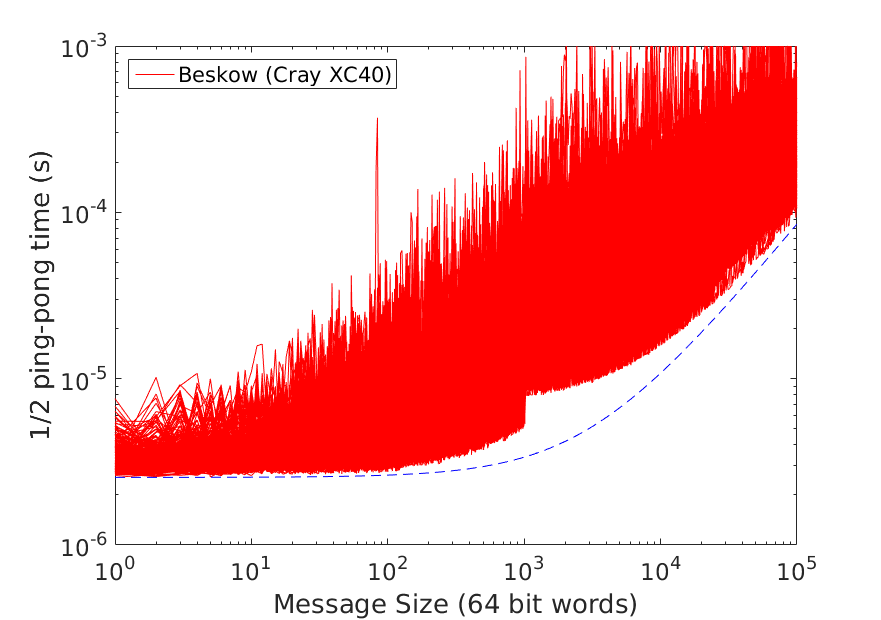
\includegraphics[width=\linewidth]{./figures/pingpong_beskow.png}
  \label{fig:pingpong_beskow}
  }
  \subfigure[Ping-pong on Titan]{
  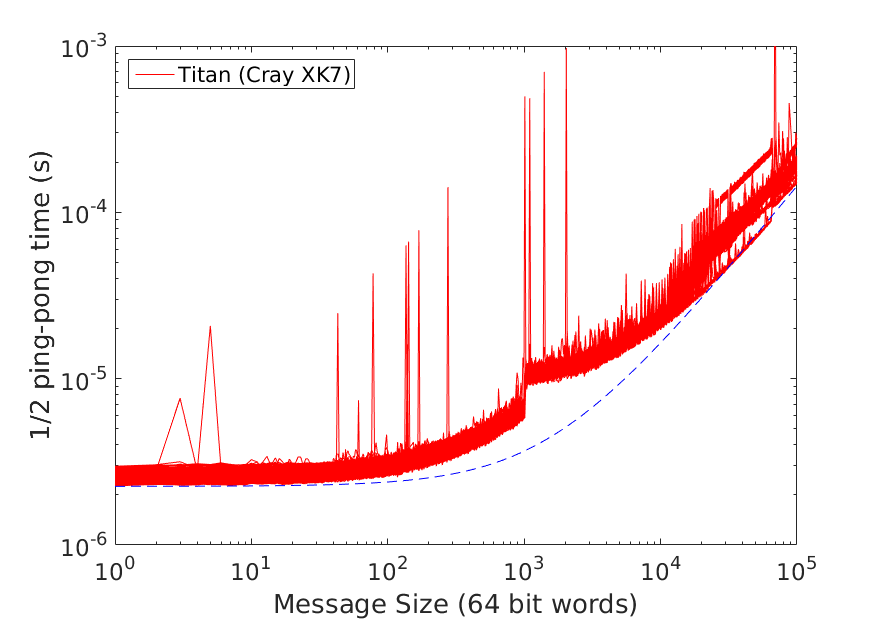
\includegraphics[width=\linewidth]{./figures/pingpong_titan.png}
  \label{fig:pingpong_titan}
  }
  \subfigure[Ping-pong and all-reduce on Mira as illustrated in \cite{fischer:scaling}]{
  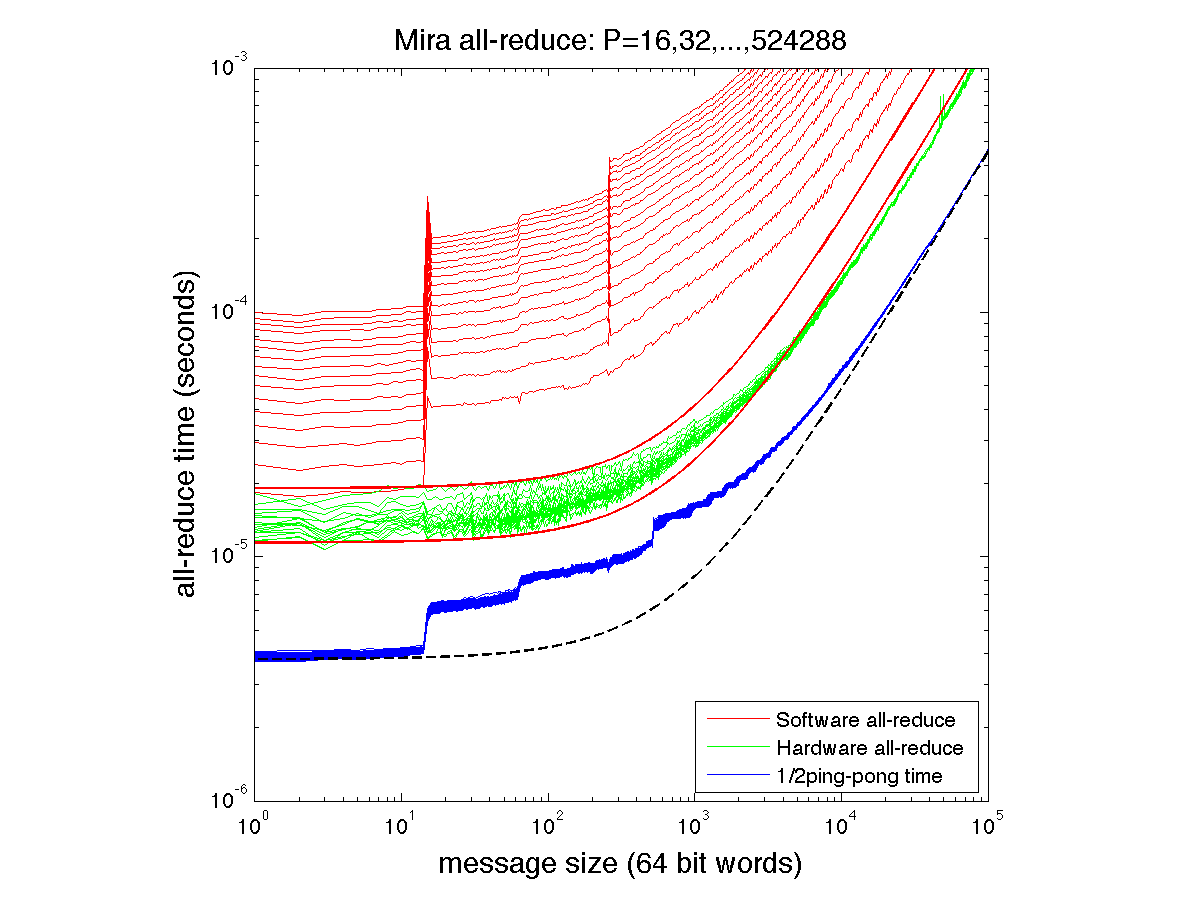
\includegraphics[width=\linewidth]{./figures/pingpong_mira.png}
  \label{fig:pingpong_mira}
  }
  \caption{Latency and Bandwidth Tests on Mira}
  \label{fig:pingpong}
\end{figure}

% Show graph with results of the ping pong test?
% Explain that we took minimum values
% Discuss noise and "randomness" of the results on Cray machines



\section{Nek5000 solver}

\subsection{Method}
projections

\subsubsection{Splitting method}
There are two main solvers available within Nek5000 for computing the solution of incompressible Navier-Stokes, of which one is also ammenable to non-divergence free flows. To preserve generality we picked the latter, based on \cite{Tomboulides1997}, which is in essence a fractional step solver. We solve the following equations
\begin{align}
 \frac{\partial \mathbf{u}}{\partial t} + (\mathbf{u \cdot \nabla}) \mathbf{u} & = - \nabla p + \frac{1}{Re} \nabla^2 \mathbf{u} + \mathbf{f} \label{eqn:NS_momentum},\\
 \nabla \cdot \mathbf{u} & = 0, \label{eqn:NS_continuity}
\end{align}
where $\mathbf{u}$ is the velocity field and $p$ the pressure. The Reynolds number $Re = \frac{U L}{\nu}$ is expressed as a function of a typical velocity scale $U$, length scale $L$ and kinematic viscosity $\nu$. Equations \refeqn{eqn:NS_momentum}  and \refeqn{eqn:NS_continuity} are called the continuity and momentum equations respectively. 

The momentum equation is time integrated via an Implicit-Explicit scheme, also known as BDFk-EXTk (Backward DiFferences and EXTrapolation of order k). We illustrate it semidiscretely

\begin{eqnarray}
\sum\limits_{j=0}^k \frac{b_j}{\Delta t} \mathbf u^{n-j}  = - \nabla p^{n}+\frac{1}{Re}\nabla^2\mathbf u^{n}+\underbrace{\sum\limits_{j=1}^k a_j [N(\mathbf u^{n-j})+\mathbf f^{n}]}_{\mathbf{F}_n(\mathbf u,\mathbf f)}\label{eqn:discrete}
\end{eqnarray}
The coefficients $b_k$ and $a_k$ are the coefficients for the explicit discretization of the time derivative and convective terms.

Ignoring boundary conditions and other numerical technicalities available in \cite{Tomboulides1997} 
\begin{align}
 \Delta p^{n} & = \nabla \cdot \left( -\frac{b_0}{\Delta t} \mathbf{u}^{n} + \mathbf{F}_n \left( \mathbf{u},\mathbf f \right) \right) \label{eqn:hmhz_pres}\\
 \Delta \mathbf{u}^{n+1}- \frac{b_0}{\Delta t} \mathbf{u}^{n+1}  & =  \nabla p^{n+1} + \mathbf{F}_n \left( \mathbf{u}, \mathbf f) \right. \label{eqn:hmhz_vel}
\end{align}

So as it can be observed solving the incompressible Navier-Stokes equations is reduced to the evaluation of $\mathbf{F}_n$ in \refeqn{eqn:discrete}, followed by one Poisson equation and a Helmholtz equation thereafter. 
Equation \refeqn{eqn:hmhz_pres}, the Poisson equation for the pressure, is the main source of stiffness and its efficient resolution by an iterative solver is preceded by two steps. First of all, the pressure at each time iteration is projected onto a subspace of previous solutions and serves as first guess for the iterative solver. We used a subspace of length $20$ in the present case. This method, described in \cite{Fischer1998}, has been shown to reduce the iteration count by a factor $2.5-5$. Then, a pressure preconditioner is built based on the additive overlapping Schwarz method, given by 
\begin{equation}
 M_0^{-1} := R_0^T A_{0}^{-1} R_0 + \sum_{k=1}^{K} R_k^T \tilde{A}_k^{-1} R_k.
\end{equation}
The overlapping part require local solves on each subdomain and is easily parallelized \cite{Fischer199784,Fischer2005}. The coarse grid solve is more difficult to parallelize and can be performed in two different ways. The first method is a Cholesky factorization of the matrix $A_0^{-1}$ into $XX^T$ with a convenient refactoring of the underlying matrix to maximize the sparsity pattern of $X^T$. This factorization is subsequently referred to as XXT and details regarding complexity and implementation are available in \cite{Tufo2001151}. 

The second method is an algebraic multigrid solver (AMG) that operates a smoothing, a coarsening and a interpolation operation on a predefined number of coarse grid levels. Finally, the pressure equation is solved with the generalized minimal residual method (GMRES).

In a similar way, Equation \refeqn{eqn:hmhz_vel}, the Helmholtz equation for the velocity, is solved using the conjugate gradient (CG) iterative solver with a simple Jacobi preconditioner.
% \begin{align}
%  \mathbf{u}_i^* & = \beta_0 \mathbf{u}_i^n + \beta_1 \mathbf{u}_i^{n-1} + \beta_2 \mathbf{u}_i^{n-2}, \label{eqn:extrap_vel}\\
%  \mathbf{h}_i^n & = N(\mathbf{u}_i^n) + B \mathbf{f}_i + ???, \label{eqn:rhs}\\
%  A \delta \mathbf{p}^n & = \nabla \cdot \left[ \left( \sum_{i=1}^3 \frac{-1}{Re} (\nabla \times (\nabla \times \mathbf{u}_i^*)) + B^{-1} \mathbf{h}_i^n \right) \right]\nonumber\\
%  & \quad - A \mathbf{p}^n , \label{eqn:hmhz_pres} \\
%  A \delta \mathbf{u}^{n} & = -A \mathbf{u}^{n} + \mathbf{h}_i^n \label{eqn:hmhz_vel},\\
%  \mathbf{p}^{n+1} &= \mathbf{p}^{n} + \mathbf{\delta p}^{n}, \label{eqn:update_p} \\
%  \mathbf{u}_i^{n+1}& = \mathbf{u}_i^{n} + \mathbf{\delta u}_i^{n}.  \label{eqn:update_u} 
% \end{align}
% The operators $A$ and $B$ represent the discrete Laplacian operator and the mass matrix respectively. The index $i=1,2,3$ represents the 3 spatial directions $x$, $y$ and $z$. The intermediate velocity $\mathbf{u}_i^*$ is extrapolated using a third order Adams-Bashforth scheme in Equation (\refeqn{eqn:extrap_vel}). The corresponding coefficients $\beta_k$ are given by $\beta_0 = \frac{23}{12}$, $\beta_1 = \frac{-4}{3}$ and $\beta_2 = \frac{5}{12}$ (??). The term $\mathbf{h}_i^n$ from equation (\refeqn{eqn:rhs}) contains the nonlinear convective term $N(\mathbf{u}_i^n)$ evaluated explicitely, the external forcing $\mathbf{f}_i$ and ???. Equation (\refeqn{eqn:hmhz_pres}) is solved using a Generalized minimal residual method (GMRES), while equation (\refeqn{eqn:hmhz_vel}) is solved using the conjugate gradient (CG) mehtod. Furthermore, both the pressure and velocity vectors are projected onto a space of previous solutions in order to speed up the convergence of the iterative solvers. Projections occur before and after the 
% iterative solver. %When solving equations (\refeqn{eqn:hmhz_pres}) and (\refeqn{eqn:hmhz_vel}), we obtain the corrections for the pressure and the velocity that we can use to update those variables in Equations \refeqn{eqn:update_p} and \refeqn{eqn:update_u}.

%\subsubsection{Coarse grid solver}

% introduce coarse grid solver for the pressure

\subsection{Implementation}
\label{sec:implementation}
The geometry is meshed using hexahedral elements, partioned for parallel computation using a spectral bisection algorithm as implemented in "genmap" which accompanies the code Nek5000 \cite{argonne:nekdoc}. An example of the repartion for the case $Re_{\tau} = 180$ run on $64$ cores is shown in \reffig{fig:partition_vis}. In this picture, each element is colored according to the MPI rank it belongs to.
\begin{figure}
  \centering
  \subfigure[Partition]{
  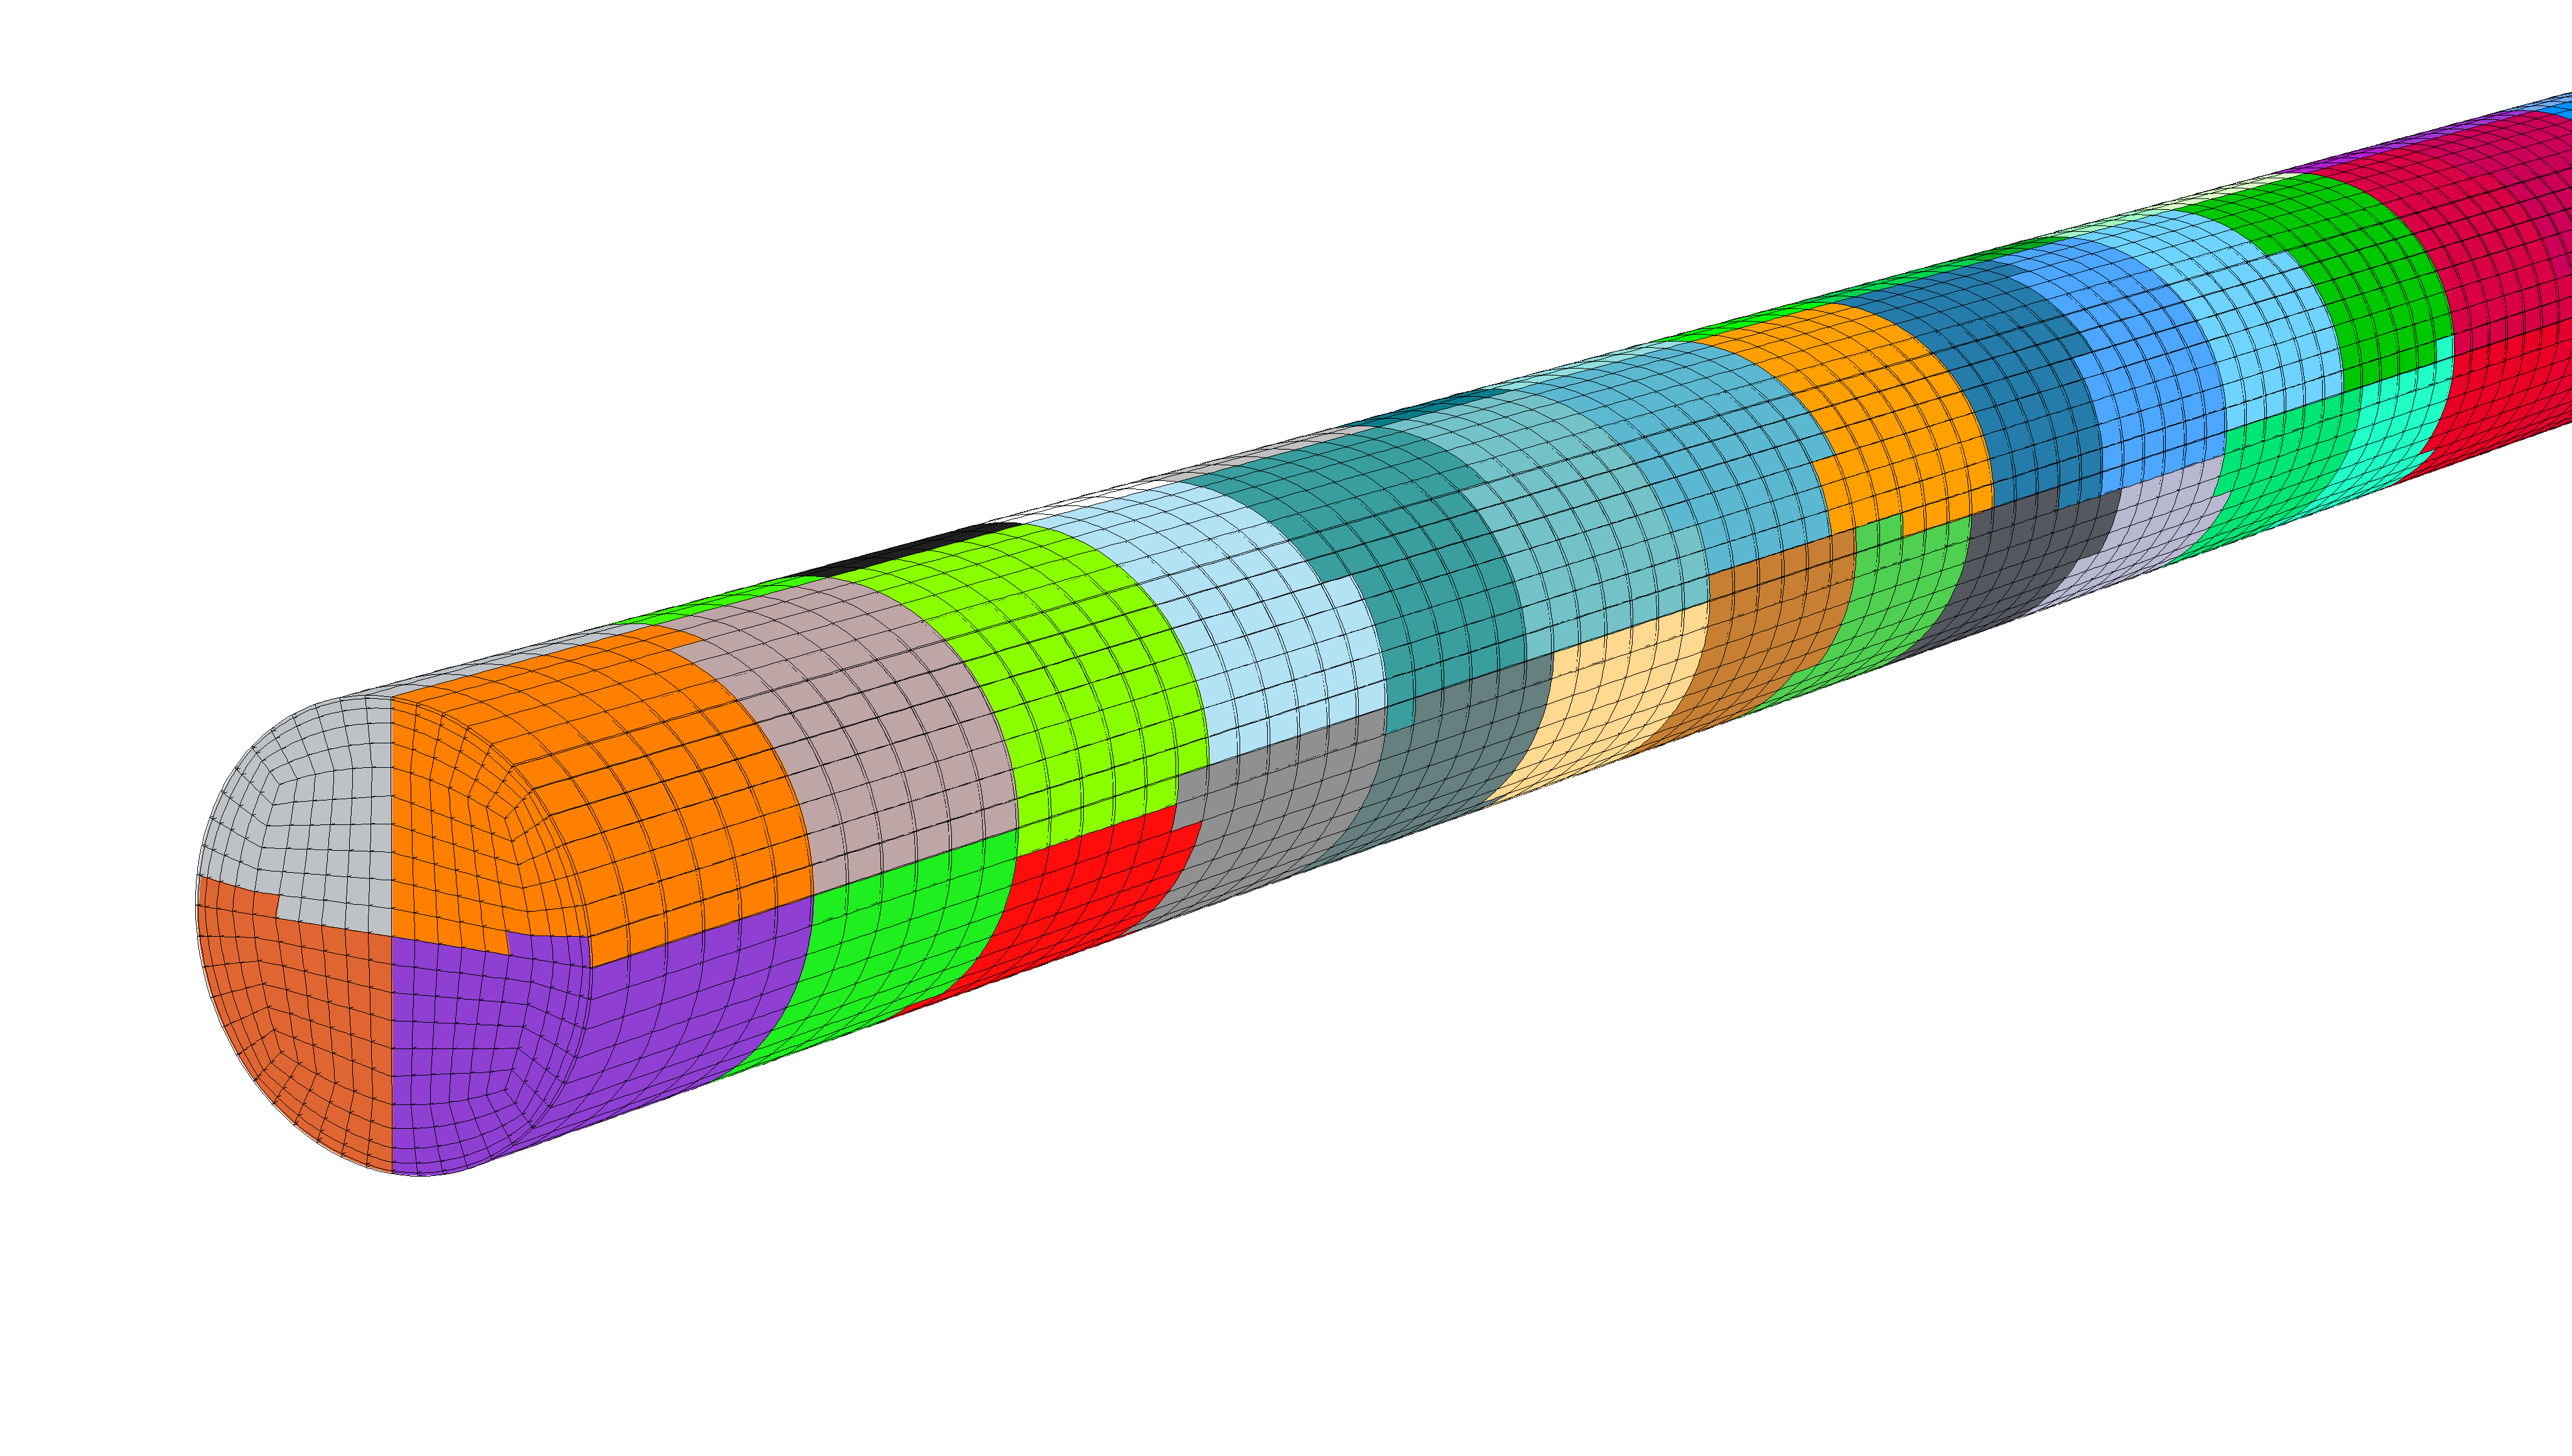
\includegraphics[trim=300 400 800 350,clip,width=\linewidth]{./figures/partition2.png}
  \label{fig:partition_vis}
  }
  \subfigure[Velocity magnitude]{
  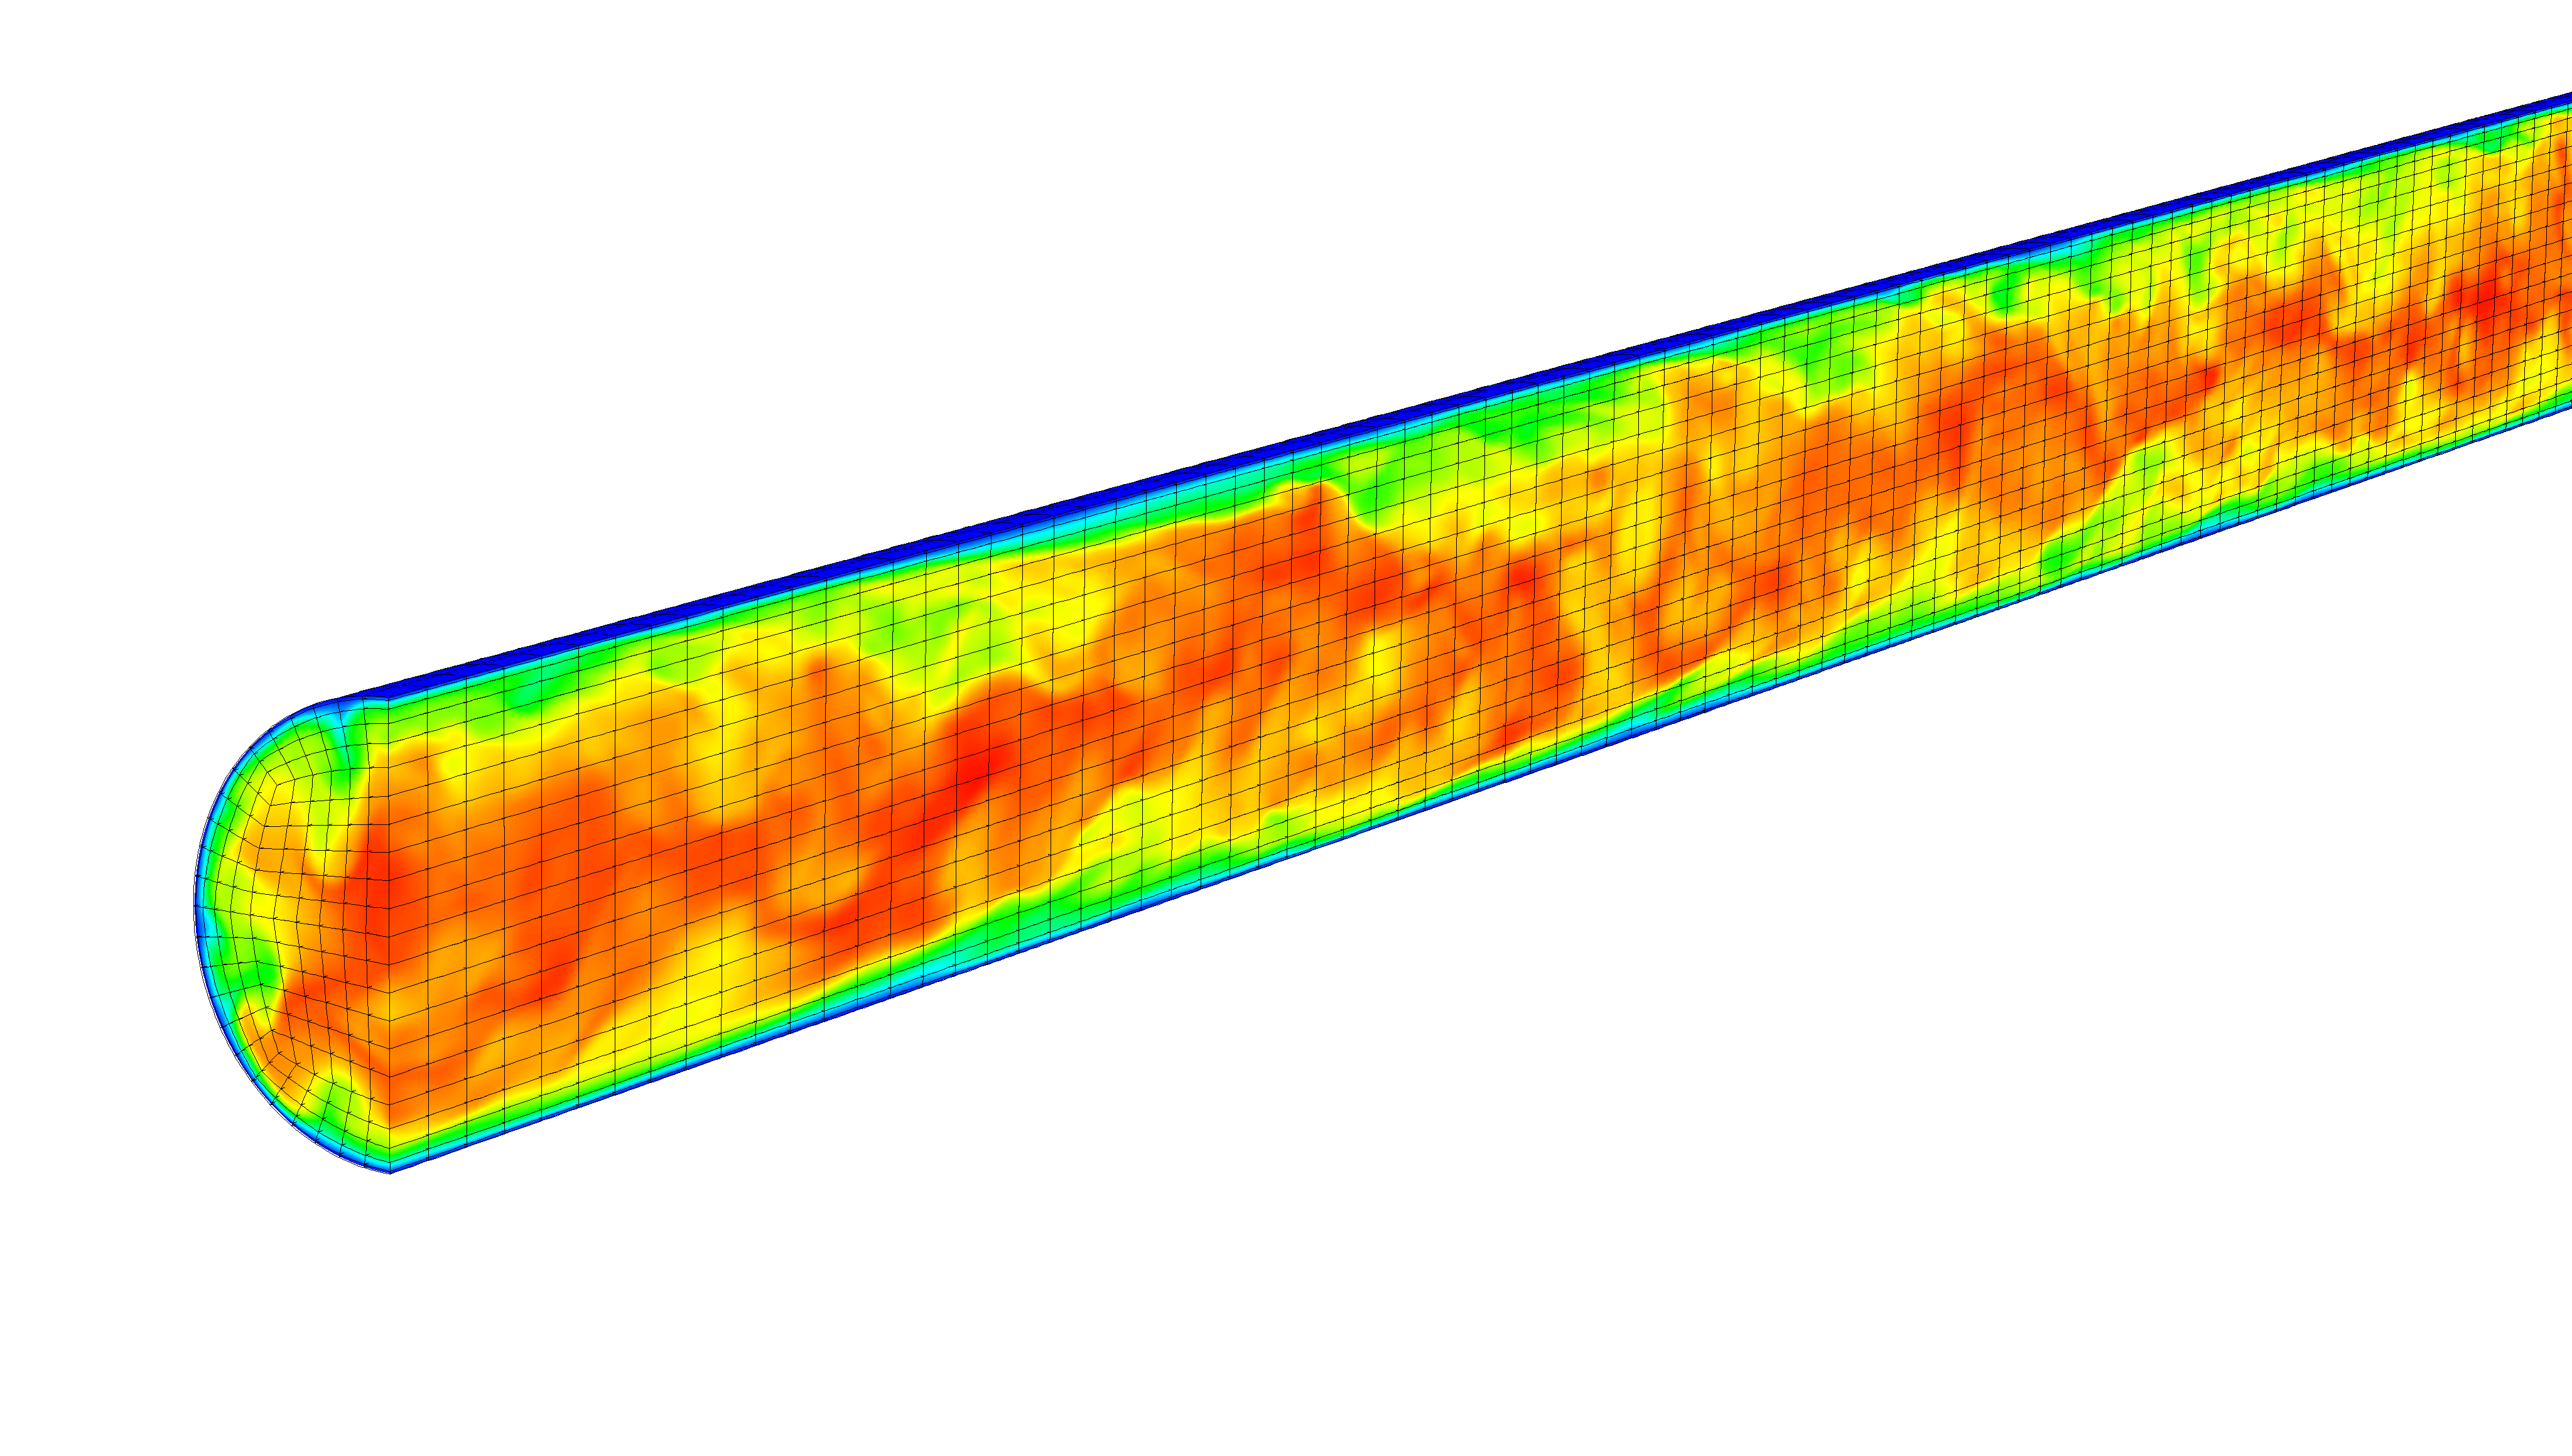
\includegraphics[trim=300 400 800 350,clip,width=\linewidth]{./figures/vel_magn.png}
  \label{fig:flow_vis}
  }
  \caption{Partition of the elements and velocity magnitude in the pipe ($Re_{\tau}=180$).}
  \label{fig:partition}
\end{figure}
 
\subsubsection{Code structure}
\label{sec:code}

The structure for solving the equations \refeqn{eqn:hmhz_pres} and \refeqn{eqn:hmhz_vel} is illustrated in \refalg{alg:code_struct}. The main loop iterates over the time steps. At each time step, the pressure is solved first and then the velocity components. We can write equations \refeqn{eqn:hmhz_pres} and \refeqn{eqn:hmhz_vel} in discrete form as 
\begin{align}
H_p \; p = r_p, \\
H_{\mathbf{u}} \; \mathbf{u} = r_{\mathbf{u}}.
\end{align}
$H_p$ and $H_{\mathbf{u}}$ are the Helmholtz operators for pressure and velocity respectively, while $r_p$ and $r_{\mathbf{u}}$ are the corresponding right hand sides or residuals. The first step to compute the solution of both fields is to compute the corresponding right hand side. The this right hand side is projected onto a subspace of previous solutions (subspaces are denoted by $X$). Then, the corrections $\delta p$ and $\delta \mathbf{u}$ are computed by solving the Helmholtz equation for the rejection of the right hand side. A simplified structure for the Helmholtz solver is shown in \refalg{alg:helmholtz}. During the Helmholtz solve, the pressure is solved with the GMRES method while conjugate gradient is used for the velocity. The pressure solve also includes the computation of the preconditioner based on the Schwarz overlapping method and coarse grid solve, which is not the case for the velocity and constitutes an important part of the work and communication.
\begin{algorithm}
\caption{PNPN method.}\label{alg:code_struct}
\begin{algorithmic}
\Procedure{Solver}{}
\For {k=1,...,nsteps} \Comment{$ttotal$}
\State \# \textbf{Compute Pressure}
\State $r_p \leftarrow rhs_p(\mathbf{u}, \mathbf{f})$ \Comment{$trhsp$}
\State $\delta r_p \leftarrow r_p - \text{proj}_{X_{r_p}}(r_p)$ \Comment{$tprojp1$}
\State $\delta p \leftarrow \text{Helmholtz}(H_p,\delta r_p)$ \Comment{$thmhp$}
\State $p \leftarrow p + \delta p$ \Comment{$tprojp2$}
\State $X_p \leftarrow \left\{ X_p, \text{proj}_{X_{p}}(p) \right\}$ \Comment{$tprojp2$}
\State $X_{r_p} \leftarrow \left\{ X_{r_p}, \text{proj}_{X_{r_p}}(H_p p) \right\}$ \Comment{$tprojp2$}
%\State $X_p, X_{r_p} \leftarrow \text{Update subspaces}(X_p, X_{r_p})$ 
\State \# \textbf{Compute Velocity}
\State $r_{\mathbf{u}} \leftarrow rhs_{\mathbf{u}}(p, \mathbf{u}, \mathbf{f})$ \Comment{$trhsv$}
\State $\delta r_{\mathbf{u}} \leftarrow r_{\mathbf{u}} - \text{proj}_{X_{r_{\mathbf{u}}}}(r_{\mathbf{u}})$ \Comment{$tprojv1$}
\State $\delta {\mathbf{u}} \leftarrow \text{Helmholtz}(H_{\mathbf{u}},\delta r_{\mathbf{u}})$ \Comment{$thmhv$}
\State ${\mathbf{u}} \leftarrow \mathbf{u} + \delta \mathbf{u}$ \Comment{$tprojv2$}
\State $X_{\mathbf{u}} \leftarrow \left\{ X_{\mathbf{u}}, \text{proj}_{X_{\mathbf{u}}}(\mathbf{u}) \right\}$ \Comment{$tprojv2$}
\State $X_{r_{\mathbf{u}}} \leftarrow \left\{ X_{r_{\mathbf{u}}}, \text{proj}_{X_{r_\mathbf{u}}}(H_{\mathbf{u}} \mathbf{u}) \right\}$ \Comment{$tprojv2$}
%\State $X_{\mathbf{u}}, X_{r_{\mathbf{u}}} \leftarrow \text{Update subspaces}(X_{\mathbf{u}}, X_{r_{\mathbf{u}}})$ 
\EndFor
\EndProcedure
\end{algorithmic}
\end{algorithm}

\begin{algorithm}
\caption{Helmholtz solve.}\label{alg:helmholtz}
\begin{algorithmic}
\Procedure{Helmholtz}{$H, r$}
\If {Velocity}
\State $x \leftarrow CG(H, r)$
\ElsIf {Pressure}
\State $\left(M_0^{-1}\right)_{\text{Sch}} \leftarrow$ Overlapping Schwarz()
\State $\left(M_0^{-1}\right)_{\text{cgs}} \leftarrow$ Coarse grid solve() \Comment{$tcoarse$}
\State $M_0^{-1} \leftarrow \left(M_0^{-1}\right)_{\text{Sch}} + \left(M_0^{-1}\right)_{\text{cgs}}$
\State $x \leftarrow GMRES(M_0^{-1}, H, r)$
\EndIf
\State \textbf{return} x
\EndProcedure
\end{algorithmic}
\end{algorithm}

\subsubsection{Instrumentation for the Timers}
\label{sec:timers}
Our strategy for timing the code execution is twofold. For one, we use MPI
timers for the wall clock time and profiling libraries that were deemed suitable
for our use case. We are running the code on our test case (see
\refsec{sec:pipe}) after a full restart for 50 time steps. We save 5 past
projections and are measuring the time from the 30th to the 50th time step; in
total 20 time steps. 
\paragraph{MPI Timers}
Based on the structure presented in \refsec{sec:code} we placed 10 timers in the code that are
only switched on during the last 20 time steps. Each timer measures the wall
clock time using the MPI timer ({\tt MPI\_Wtime}) followed by a barrier
({\tt MPI\_Barrier}) guaranteeing coherent and synchronized measurements. We
have run the code without synchronization and timers to evaluate the created
overhead due to our measurements. In all instances this overhead has been far
below 5\%. The main timer ($ttotal$) measures the total time spent in the outer timestepping loop for the last 20 timesteps. Then, we have timers for the compute time of the right hand side of equation \refeqn{eqn:hmhz_pres} ($trhsp$), and of the right hand side of equation \refeqn{eqn:hmhz_vel} ($trhsv$). We also time all the different projections separately, using two timers for both the pressure and velocity: one timer for projecting the residuals before the Helmholtz solve ($tprojp1$ and $tprojv1$) and one for updating and projecting the field after the solve ($tprojp2$ and $tprojv2$). The timer for this second projection step also includes the time to update the subspaces. The time spent in the Helmholtz solves is measured as well for pressure and velocity ($thmhp$ and $thmhv$). Within the pressure solver, we put a timer around the coarse grid solve ($tcoarse$). Finally, we gather in an additional timer most of the remaining computations such that our timers account for more that 95\% of the total time. We learn from these timers that the projections are in most cases the most time consuming functions, followed by the Helmholtz solves. However, these timers do not provide information about the repartition between the time spent in computation and communication, which is the core element when assessing scalability and efficiency of a parallel code. Therefore, we do not present the results obtained with those timers and instead investigate in more details the timings produced by more adapted sampling and profiling tools.
\paragraph{Craypat and Hardware Performance Monitor}
In order to measure the time spent in communication we relied on Craypat for
Beskow and Titan and on Hardware Performance Monitor (HPM) for Mira. Both tools
allow us to measure the total time spent in communication during the targeted 20 time
steps. In addition HPM gives additional information on the cache misses and the load
imbalance. The CrayPat performance analysis framework is used to sample the code during execution at a default frequency of $\unit[100]{Hz}$ and reports in which function each sample was taken. Then, we assume that the proportion of the total time spent in a given function is equal to the proportion of samples within this function. The sampling procedure ensures a very low overhead. We also tested the profiling procedure, where all function calls are tracked, available with Craypat but overhead in time was about $50\%$ and the method was abandoned.

%\subsection{Models for parallel performance}

%\subsubsection{Computational complexity}

%\subsubsection{Communication model}

% In practice, each simulation is restarted from a previously computed turbulent solution and is run during $50$ time steps. The projections for velocity and pressure are turned on after $5$ time steps, the number of the previous pressure solutions saved is $20$ and the timers are turned on during the last $20$ time steps. Therefore, heavy input/output is not included and projections are working fully during the measurement period.

% Present system of equations
% Describe briefly the algorithm behind nek
% Mention and discuss PN-PN
% Discuss the two coarse grid solver XXT and AMG

\section{Performance and Scaling Analysis}
\label{sec:analysis}
We assume that large scale runtime performance is influenced mainly by 
\begin{enumerate}
  \item Network topology, \label{enum:a}
  \item Time $T_a$ and $T_c$ spent in computation and communication,
    respectively, as well as latency and bandwidth\label{enum:b},
  \item ratio of runtime and communication times: $r \leq \dfrac{T_a}{T_c}$,\label{enum:c}
  \item degrees of freedom $N$ per process $P$: $\dfrac{N}{P}$,\label{enum:d}
  \item and partitioning imbalance.\label{enum:e}
\end{enumerate}

The partitioning for our test case (see \refsec{sec:pipe}) is considered to be
topologically equivalent to a cube. The resulting runtime complexities are
extensively described in \cite{fischer:scaling}. We avoid to discussion of
mapping efficiently complex partitionings on network topologies and focus on
extracting insight on \ref{enum:b} to \ref{enum:e} from our conducted runs. Our
profiling tools and wall clock timers allow us to measure the load imbalance,
cache misses, as well as weak and strong scaling. Load imbalance and cache
misses are only measured on Mira via the HPM profiling library. 
While relying on the results of \cite{tufo:terascale}, we want in particular to verify
experimentally the strong scaling limit which is defined as the ratio of $\dfrac{N}{P}$ where
$\dfrac{T_a}{T_c}\leq 1$ inequality is equal to $1$ with increasing $P$. 
A generic case, widely known across the CFD community, is used to explore the
scaling behavior of Nek. This should allow potential users to estimate and
compare the scaling of Nek to other CFD software.
Our test case is run in four different regimes at 4 different problem sizes called
$Re_{\tau} 180, Re_{\tau} 360, Re_{\tau} 550, Re_{\tau} 1000$ described more in
detail in the next section.
\subsection{Test Case: Pipe}
\label{sec:pipe}

The test case considered is the turbulent flow in a straight pipe. A thorough description of the flow configuration as well as a detailed analysis of the physical results can be found in \cite{Khoury2013}. The flow was run at four different friction Reynolds numbers $Re_{\tau} = 180$, $360$, $550$ and $1000$. A summary of the different simulations and associated number of elements and number of grid points is presented in Table \reftab{tab:pipe_conf}. The friction Reynolds number is defined as $Re_{\tau} = u_{\tau} R / \nu$, where $u_{\tau}$ is the friction velocity $R$ is the radius of the pipe and  $\nu$ is the kinematic viscosity. The bulk Reynolds number is defined as $Re_{b} = 2 U_b R / \nu$, where $U_b$ is the mean bulk velocity. A snapshot of the velocity magnitude for the case $Re_{\tau} = 180$ is illustrated in \reffig{fig:flow_vis}.

\begin{table}
\centering
\caption{Summary of the different pipe flows configurations.}
\begin{tabular}{llrr} 
\hline
$Re_{\tau}$&$Re_{b}$&\# of elements & \# of grid points\\ 
\hline
$180$ & $5300$ & $36,480$ & $18.67 \times 10^6$\\
$360$ & $11,700$ & $237,120$ & $121.4 \times 10^6$\\ 
$550$ & $19,000$ & $823,632$ & $437.0 \times 10^6$\\ 
$1000$ & $37,700$ & $1,264,032$ & $2.184 \times 10^9$\\
\hline
\end{tabular}
\label{tab:pipe_conf}
\end{table}
%\subsection{Abstractions and Assumptions}
%\label{sec:abstractions}
%\subsubsection{$\alpha$, $\beta$}
%\subsubsection{Imbalance}
%\subsubsection{Weak/Strong Scaling, Efficiency}
%\subsubsection{Cache Misses and Scaling}
%\subsubsection{Partitioning and Imbalance}


\section{Results}

Our four test cases were run with various processor counts on three systems. The
lower bound for the processor count is given by the amount of RAM to fit a given
problem into memory. Nek5000 has roughly a memory requirement of 500 fields
times the number of degrees of freedoms. The upper bound was either due to the
administrative limit of getting access to the maximum number of processors
(Beskow and Titan) or by the limit of having 1 or 2 elements per process. As has
been pointed out in \refsec{sec:code}, the parallelization of Nek5000 is at the
element level so that one element may not be partitioned further. 
As anticipated in \refsec{sec:timers}, we measure the communication time and
computation time of the chosen 20 timesteps. 

In \cite{fischer:scaling} the strong scaling limit where $r=\dfrac{T_a}{T_c}=1$ was estimated
to be at about $\frac{n}{P}=2000$ for the conjugent gradient (CG) and $20000$ or
$7000$ (BG/Q) for the algebraic multigrid (AMG). As described in \refsec{sec:code}, the
Nek5000 solvers XXT and PNPN consist of several CG and AMG solves. Furthermore,
there is an overhead for the setup, the projections, the coarse solve and other
none runtime relevant components. Moreoever, the convergence of the underlying
algorithms is also very case dependent, thus influencing the overall runtime
behavior. Our runtimes give an overall impression of the Nek5000 behaviour on
various systems based on a generic well known case in CFD (see
\refsec{sec:pipe}). 

The scaling plots for all three
systems in \reffig{fig:scaling_mira}, \reffig{fig:scaling_titan}, and \reffig{fig:scaling_beskow} are the fundamental
measurements for our further analysis of the weak/strong scaling, computation
versus communication time and load imbalance.
\begin{figure}
  \centering
  \subfigure[$Re_{\tau} = 180$]{
  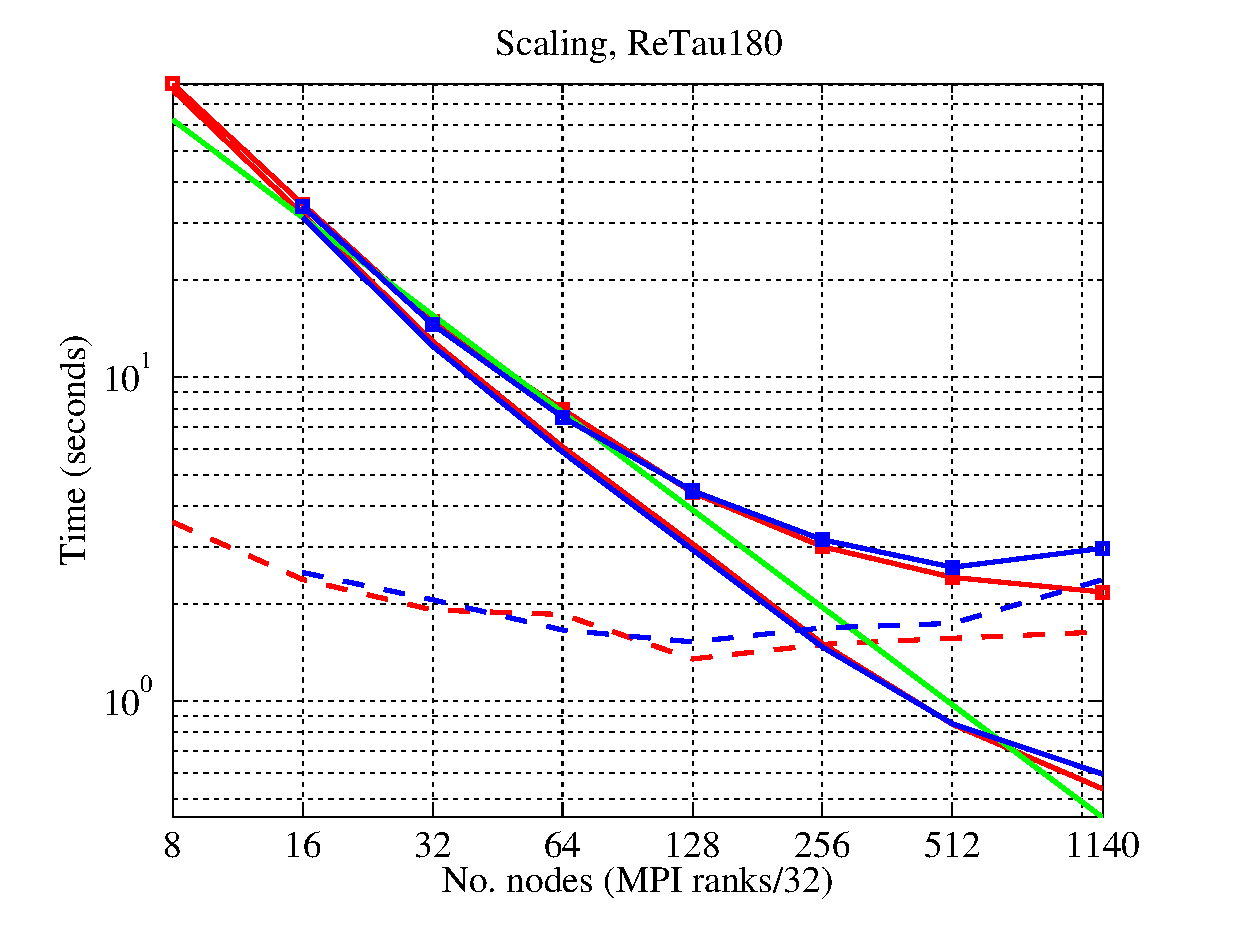
\includegraphics[width=0.85\linewidth]{./figures/mira/retau180.eps}
  }
  \subfigure[$Re_{\tau} = 360$]{
  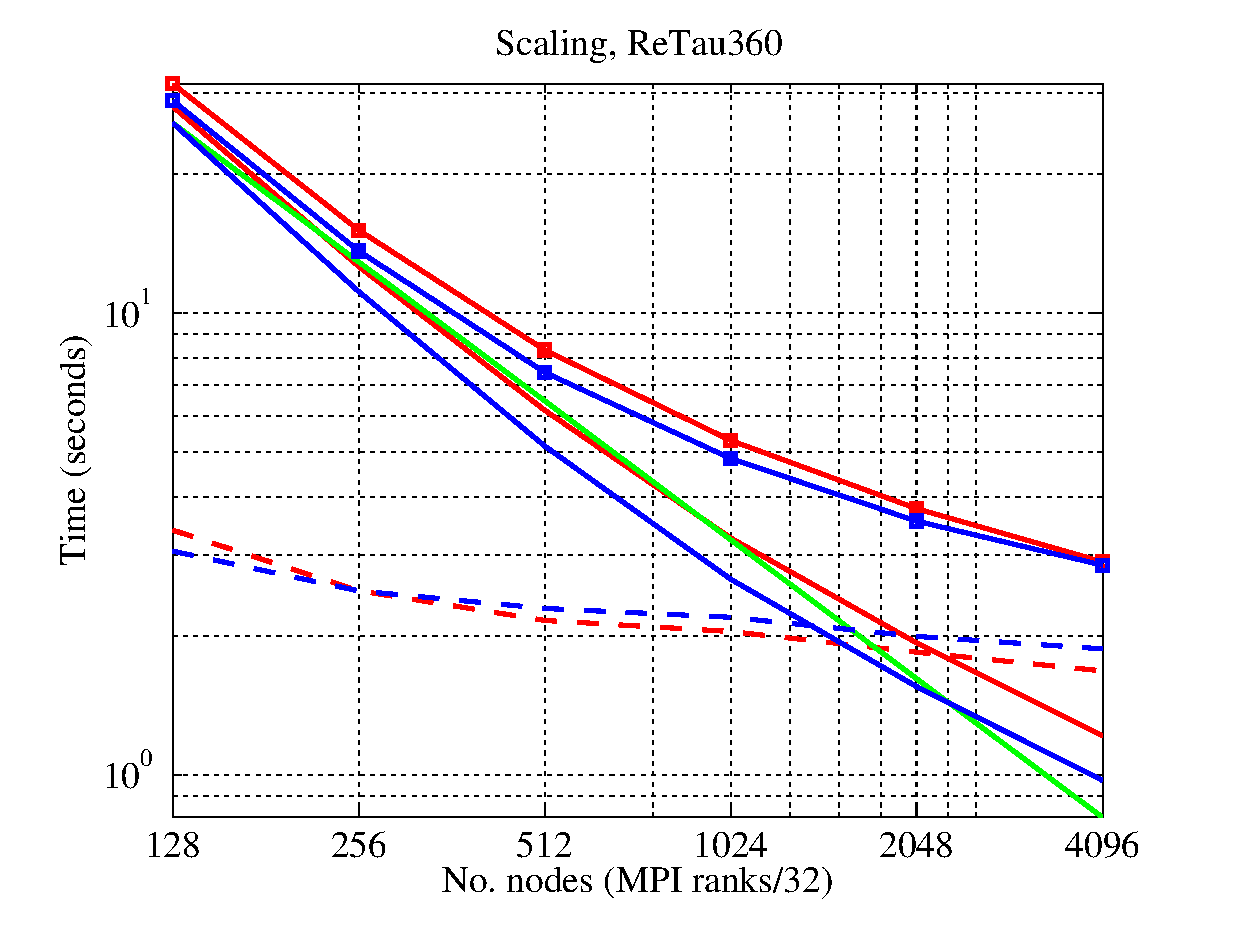
\includegraphics[width=0.85\linewidth]{./figures/mira/retau360.eps}
  }
  \subfigure[$Re_{\tau} = 550$]{
  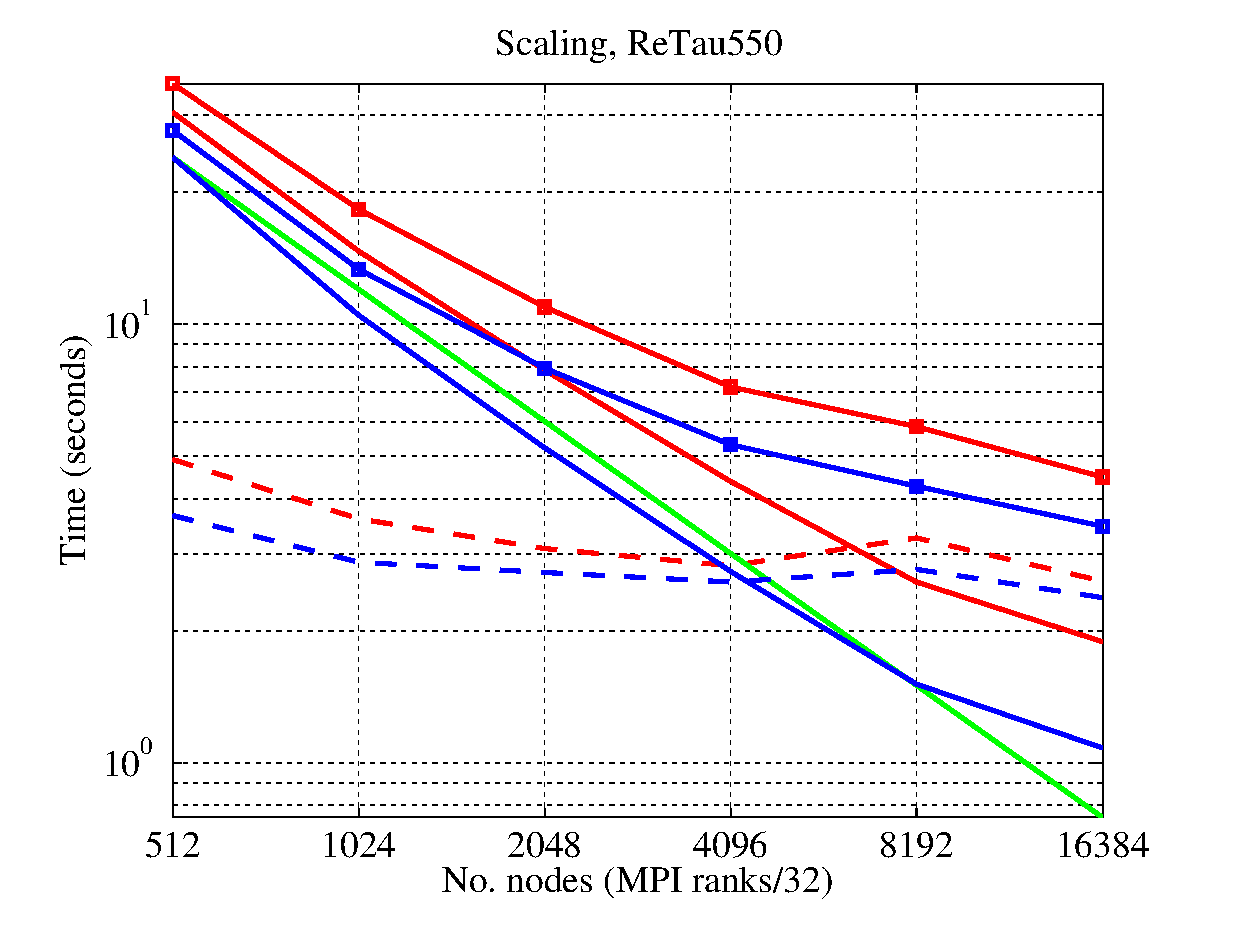
\includegraphics[width=0.85\linewidth]{./figures/mira/retau550.eps}
  }
  \subfigure[$Re_{\tau} = 1000$]{
  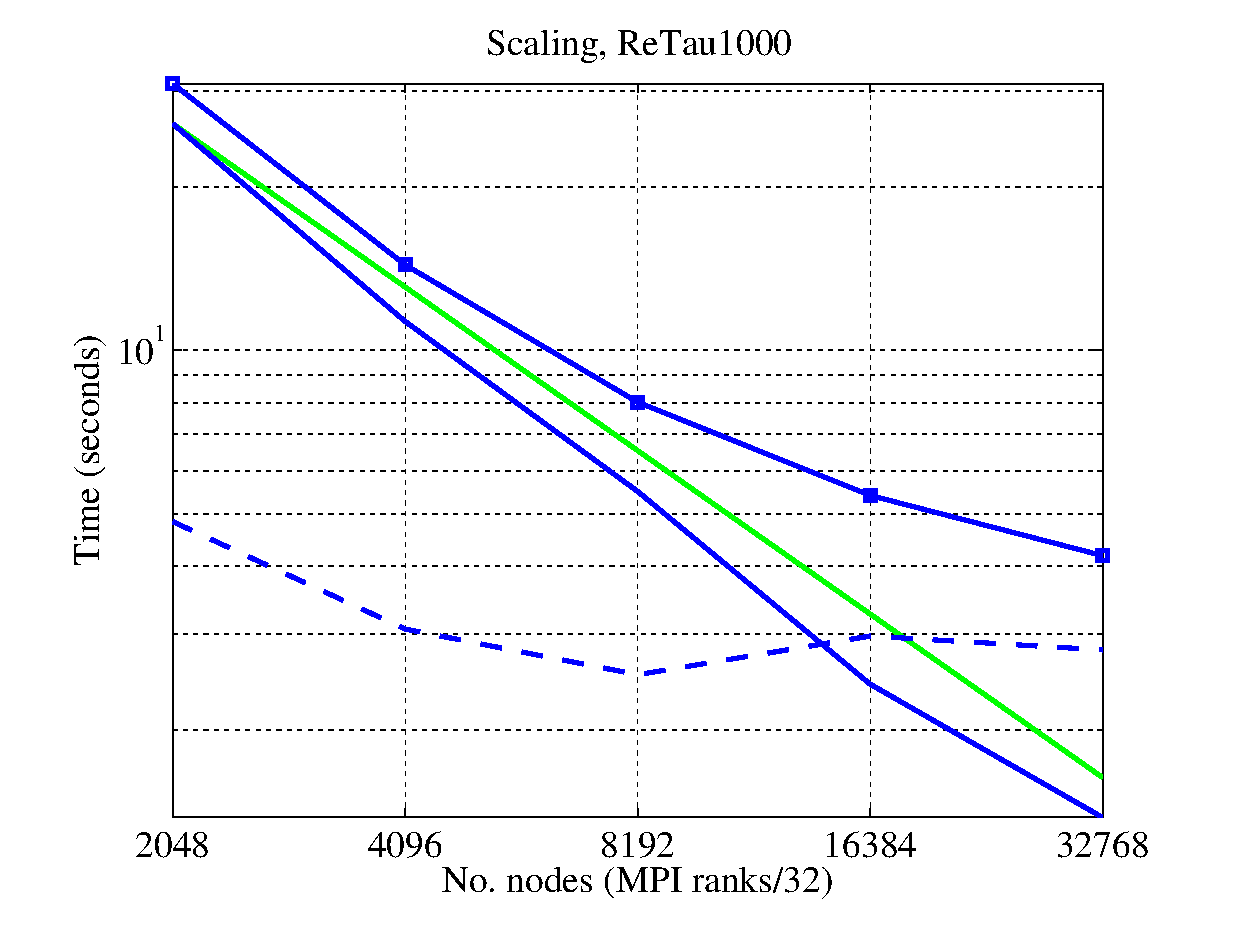
\includegraphics[width=0.85\linewidth]{./figures/mira/retau1000.eps}
  }
  \caption{BG/Q Mira}
  \label{fig:scaling_mira}
\end{figure}

\begin{figure}
  \centering
  \subfigure[$Re_{\tau} = 180$]{
  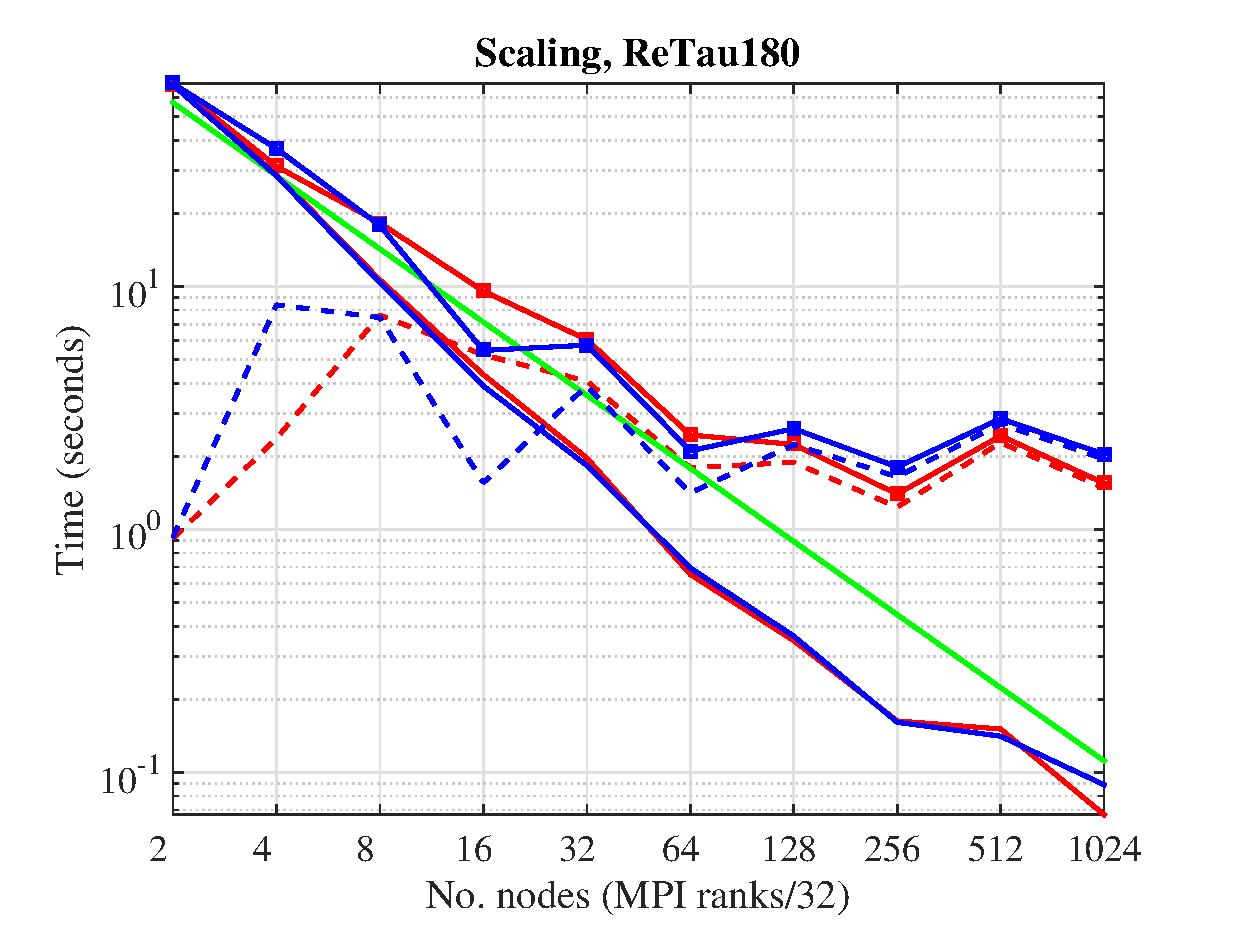
\includegraphics[width=0.85\linewidth]{./figures/beskow/scaling_ReTau180_beskow.eps}
  }
  \subfigure[$Re_{\tau} = 360$]{
  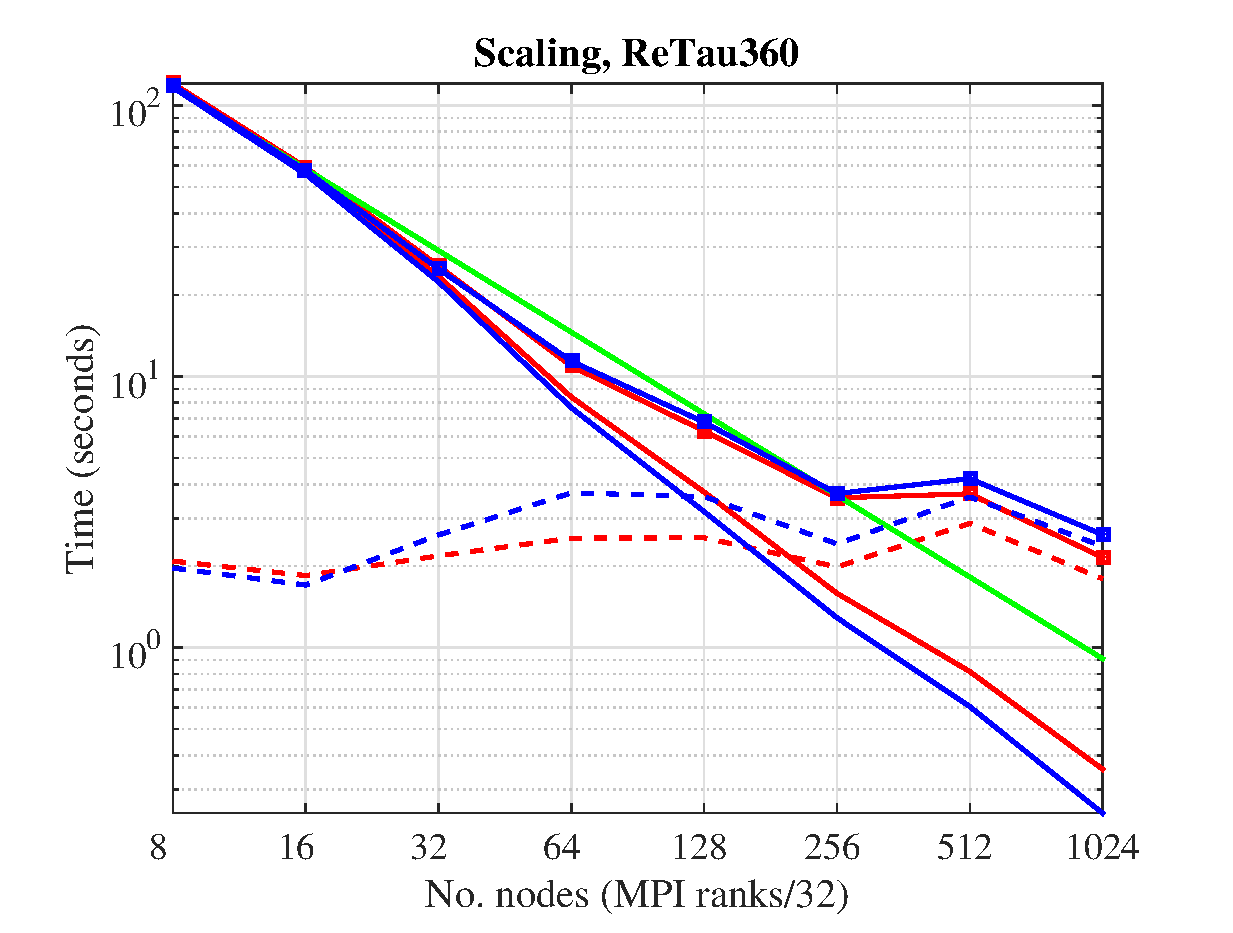
\includegraphics[width=0.85\linewidth]{./figures/beskow/scaling_ReTau360_beskow.eps}
  }
  \subfigure[$Re_{\tau} = 550$]{
  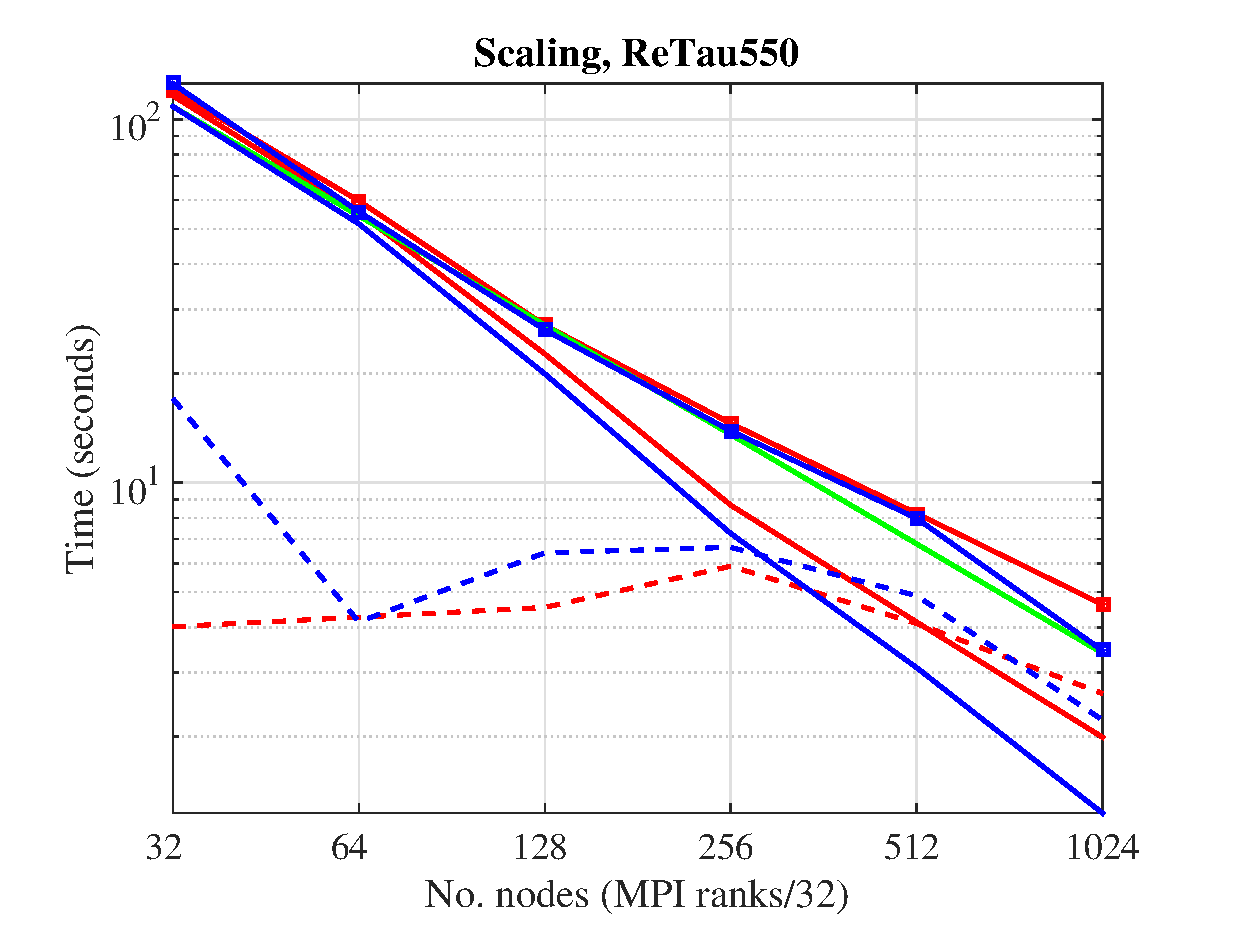
\includegraphics[width=0.85\linewidth]{./figures/beskow/scaling_ReTau550_beskow.eps}
  }
  \subfigure[$Re_{\tau} = 1000$]{
  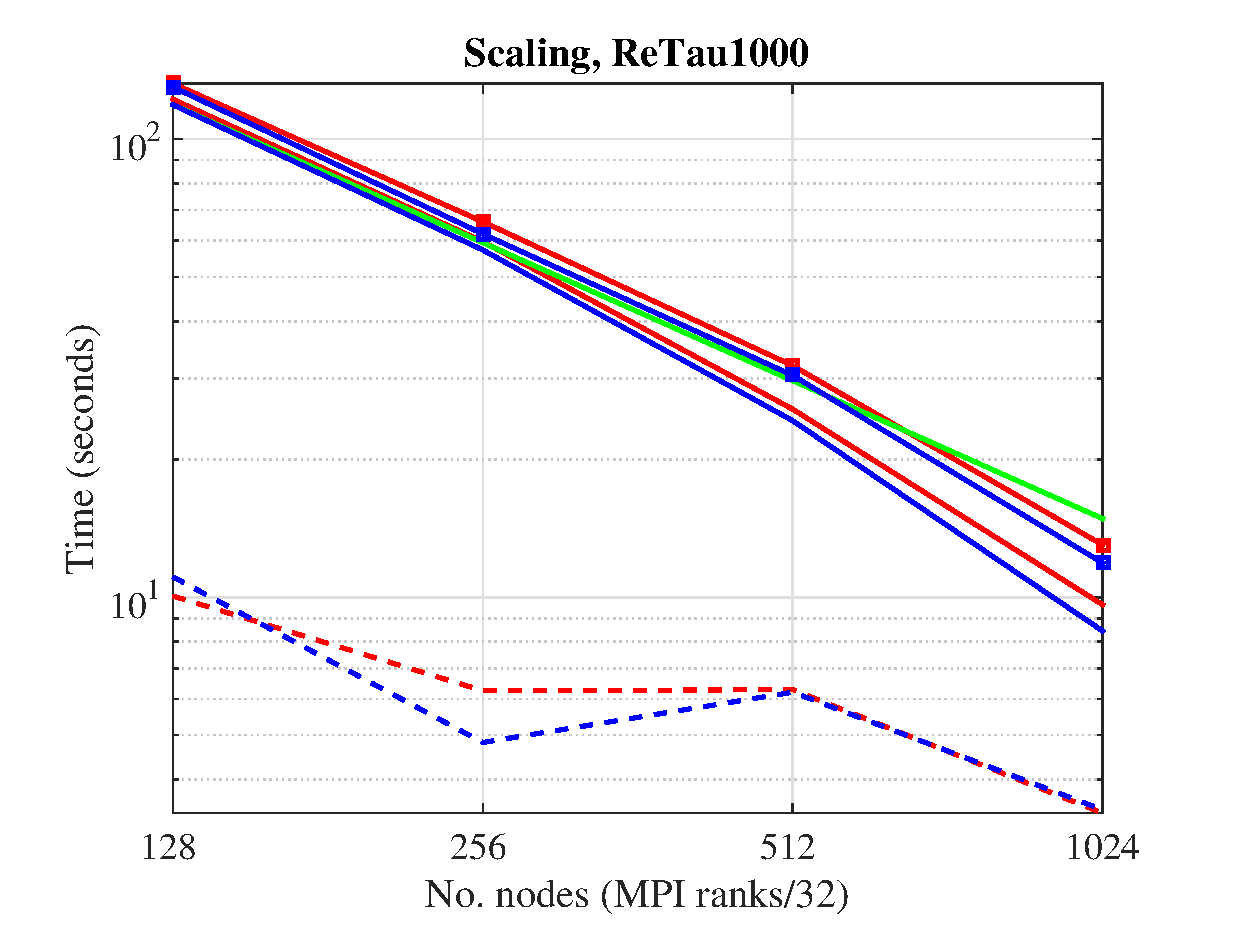
\includegraphics[width=0.85\linewidth]{./figures/beskow/scaling_ReTau1000_beskow.eps}
  }
\caption{Beskow}
\label{fig:scaling_beskow}
\end{figure}

\begin{figure}
  \centering
  \subfigure[$Re_{\tau} = 180$]{
  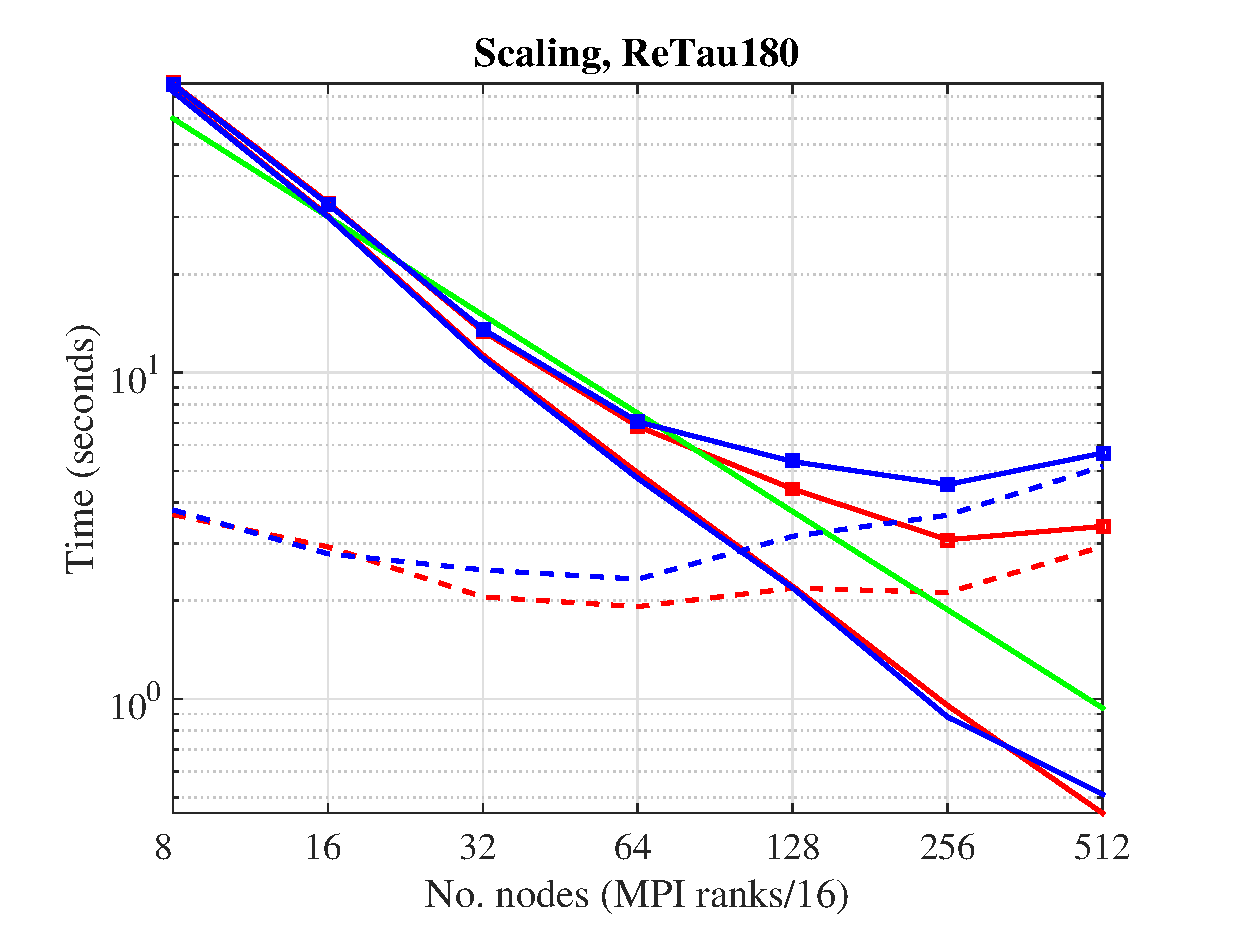
\includegraphics[width=0.85\linewidth]{./figures/titan/scaling_ReTau180_titan.eps}
  }
  \subfigure[$Re_{\tau} = 360$]{
  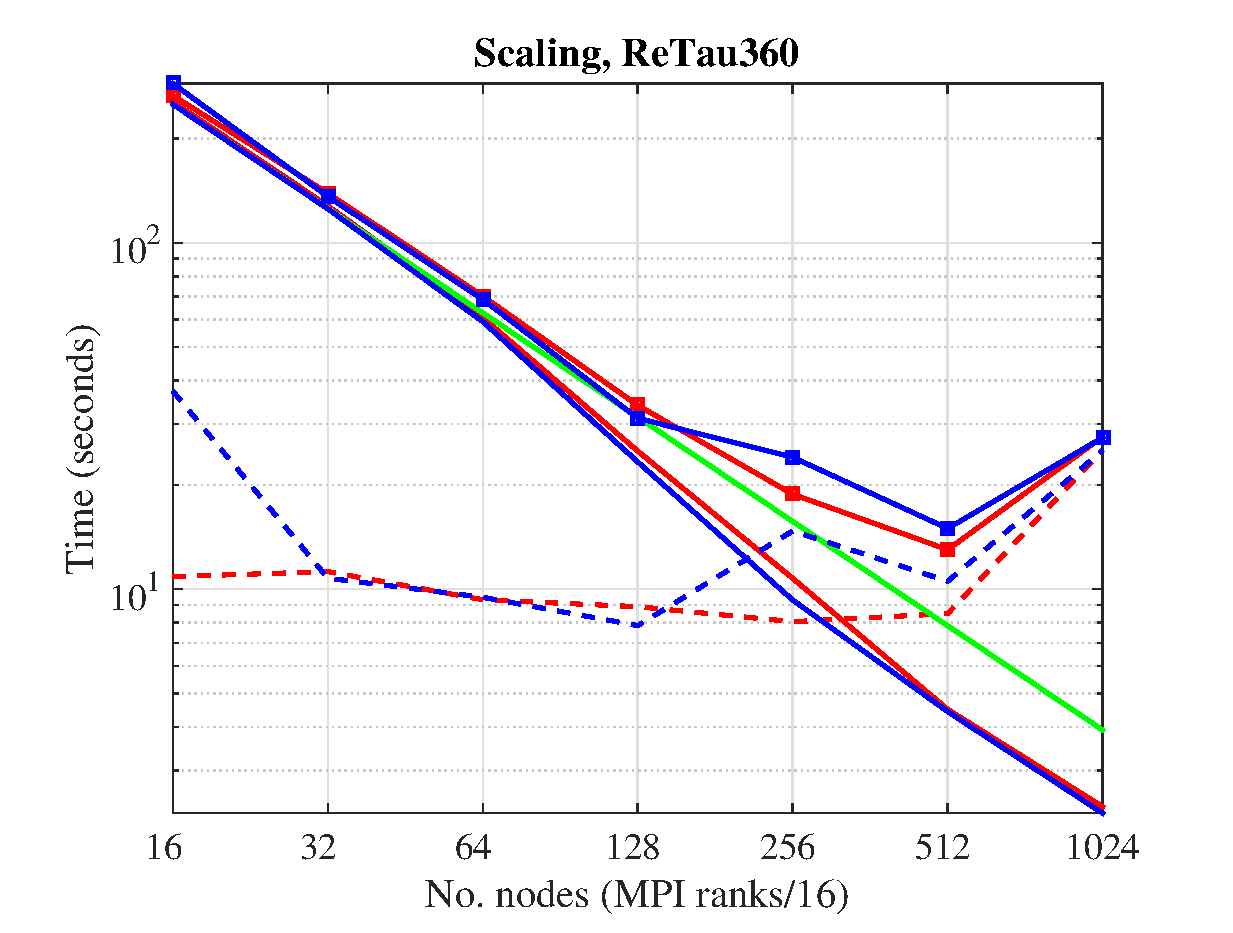
\includegraphics[width=0.85\linewidth]{./figures/titan/scaling_ReTau360_titan.eps}
  }
  \subfigure[$Re_{\tau} = 550$]{
  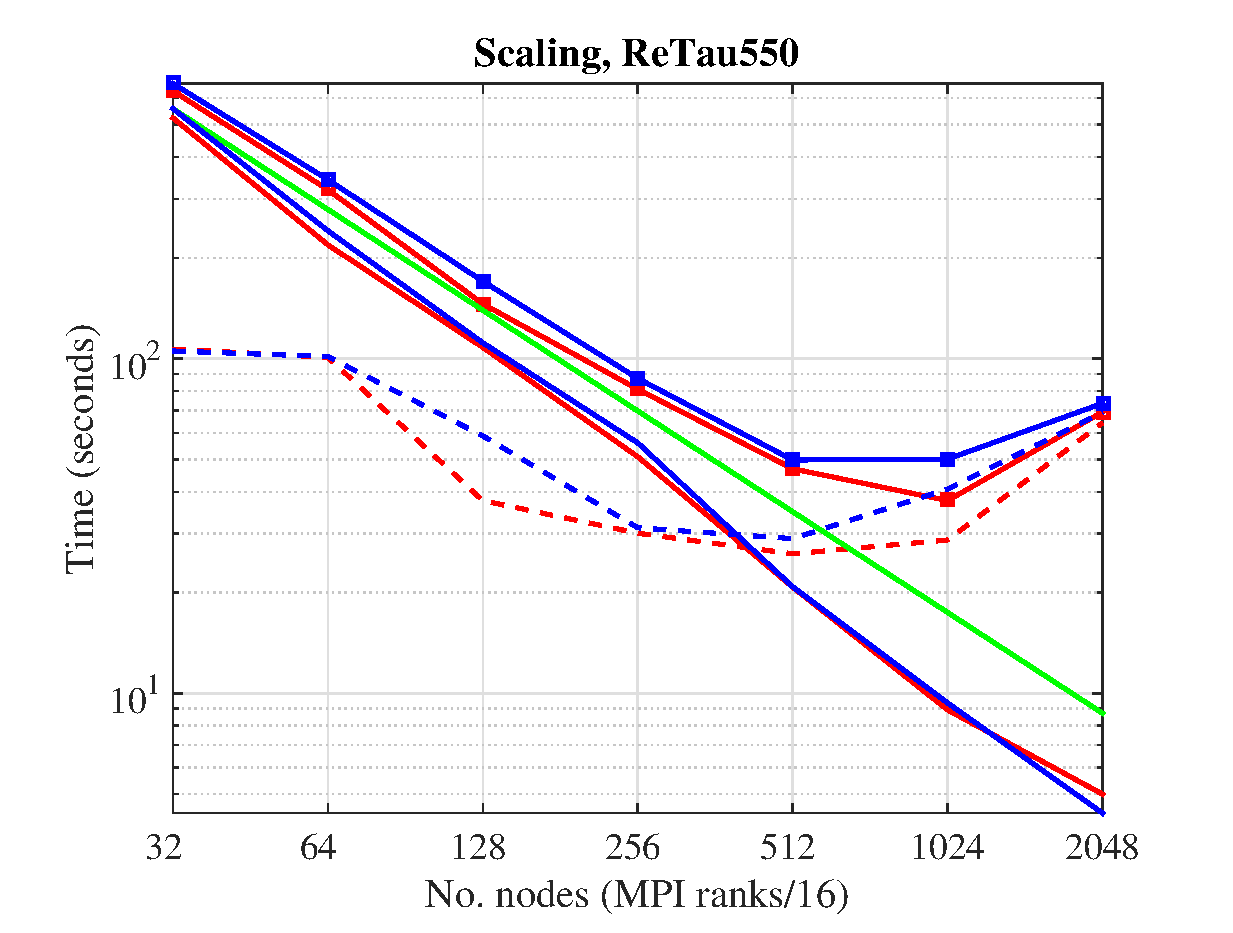
\includegraphics[width=0.85\linewidth]{./figures/titan/scaling_ReTau550_titan.eps}
  }
  \subfigure[$Re_{\tau} = 1000$]{
  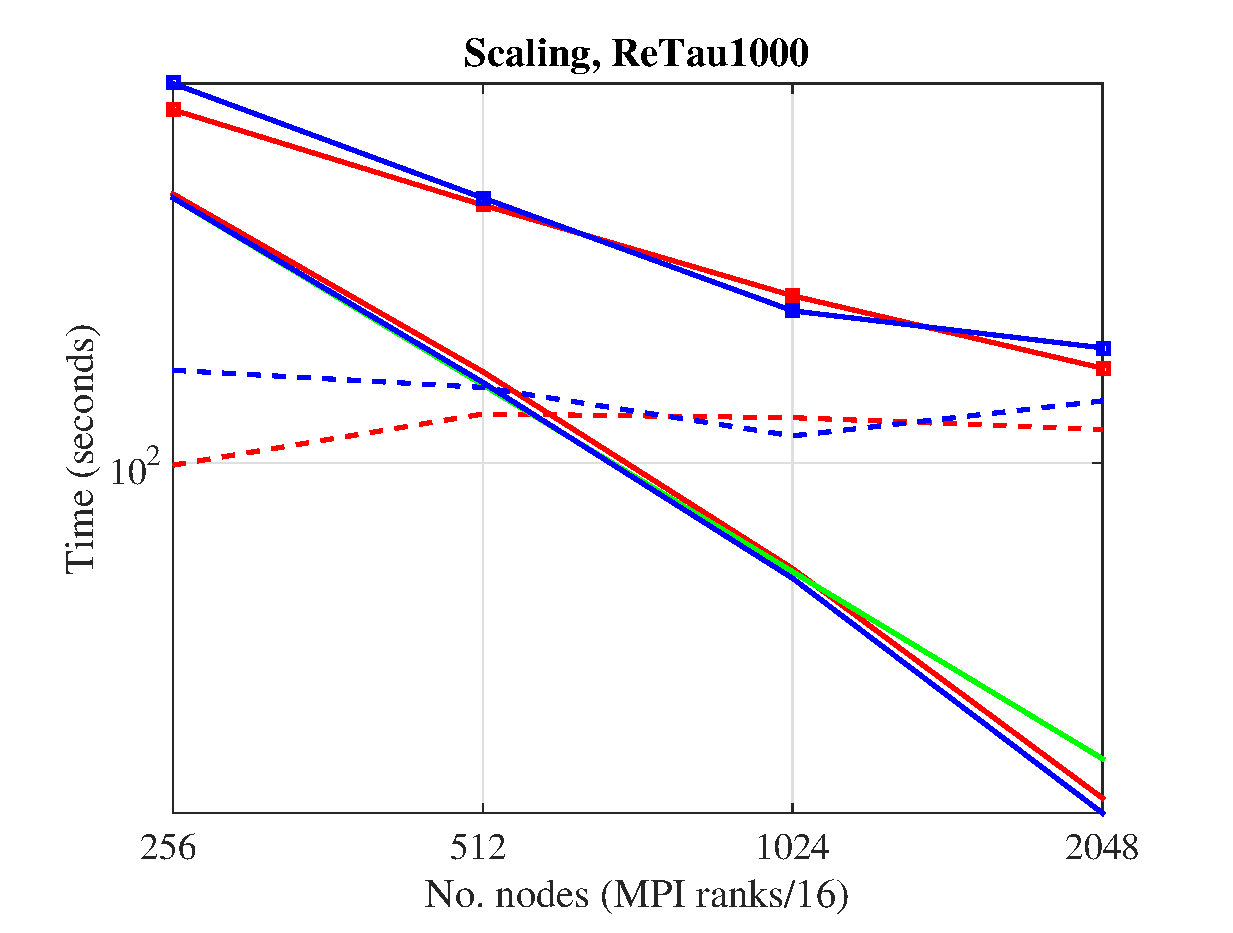
\includegraphics[width=0.85\linewidth]{./figures/titan/scaling_ReTau1000_titan.eps}
  }
\caption{Titan}
\label{fig:scaling_titan}
\end{figure}



\subsection{Weak and Strong Scaling}

The ratio of computation and communication time $r=\frac{T_a}{T_c}$ is a key
indicator for the strong scaling limit. If communication takes longer than
computation, the code is deemed to be at the strong scaling limit where the
scaling diverges significantly from the perfect linear scaling. For both XXT and
AMG this point is clearly determined in the plots where the computation time
crosses the communication time. 

\begin{table}  
  \caption{Strong Scaling Limit for all 4 test cases on Beskow, Titan and Mira
  in degrees of freedom per core $\frac{n}{P}$ with 2 processes per core on Mira, 1 process per core on Beskow and Titan}
  \begin{tabular}{c||cccc}
    \hline
    \hline
    {\bf Mira}
    &$Re_{\tau} 180$&$Re_{\tau} 360$&$Re_{\tau} 550$&$Re_{\tau} 1000$\\
    \hline
    XXT&4496&3412&4192&\\
    AMG&5040&5578&6200&9750\\
    \hline
    \hline
    {\bf Beskow}
    &$Re_{\tau} 180$&$Re_{\tau} 360$&$Re_{\tau} 550$&$Re_{\tau} 1000$\\
    \hline
    XXT&45700&19200&26000& - \\
    AMG&24800&33000&48000& - \\
    \hline
    \hline
    {\bf Titan}
    &$Re_{\tau} 180$&$Re_{\tau} 360$&$Re_{\tau} 550$&$Re_{\tau} 1000$\\
    \hline
    XXT&9000&24000&65000&228000\\
    AMG&11000&36000&68000&132000\\
    \hline
    \hline
  \end{tabular}
  \label{tab:stronglimit}
\end{table}
The approximations of values for $\frac{n}{P}$ where
$r=1$ were determined using linear intepolation (see \reftab{tab:stronglimit}).
 In practice we observed a strong scaling limit $r=1$ for XXT at roughly $1900<
\frac{n}{P} < 2300$ and for AMG at $2300<\frac{n}{P}<4000$, below the $7000$
anticipated in \cite{fischer:scaling}. 

In theory the compute time scaling should exactly match linear scaling
as computational work is distributed according to the ratio $\frac{n}{P}$. All
algorithms in Nek5000 should yield little overhead due to the halo update. 

\begin{figure}
  \centering
  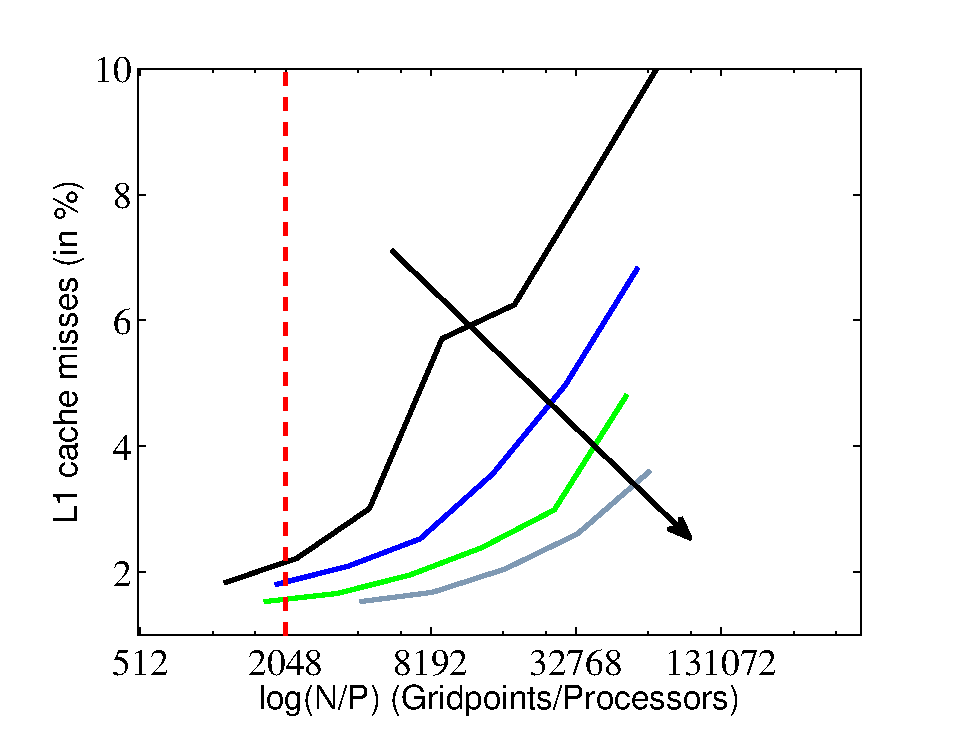
\includegraphics[width=\linewidth]{./figures/cachearrow.eps}
  \caption{Cache misses on Mira for all 4 test cases(low to high degrees of freedom in direction of the arrow) The dashed red line: L1 cache size}
   \label{fig:cachemisses}
\end{figure}

All test cases on all the systems show a super linear scaling. This
observation holds true with all timers and profilers switched off.
Numerically there is no explanation for this behavior. 

The usual explanation for super linear scaling is a sudden decrease of the cache
misses for decreasing $\frac{n}{P}$, as parts of the solver can entirely work on
data that lies in the cache. 
To investigate this, we extracted the cache misses on Mira provided by HPM (see
\reffig{fig:cachemisses}). Mira is equipped with L1 cache of 16kb. The L2 cache
of 32mb, that is located at the node level, is irrelevant as we had consistently
over 97\% cache misses. The L1 cache can be filled with $2048$ double precision, see
\reffig{fig:cachemisses} the vertical dashed redline which inidicates the cache size below which all gridpoints would theoretically fit into cache. As we run with 2 processes per core, this would be at roughly 1000
degrees of freedom per process. Although the data fields achieve those sizes only at the strong scaling
limit we do observe a general decrease in cache misses with decreasing
$\frac{n}{P}$. The only exception is the test case for $Re_{\tau}=180$ where we
have a sudden spike in cache misses where we run at one element per core. This
is the only run that was performed at a process count that is not to the power
of two.
In summary, we attribute the super linear scaling to cache
management and pipelining on the CPU of Mira. 

Comparing XXT and AMG we have a very clear picture on Mira. For smaller element
numbers XXT ($Re_{\tau} 180$) performs best and from 200k elements onwards
($Re_{\tau})$) AMG takes the lead. Although AMG has a much lower strong
scaling limit, it outperforms XXT in time to solution (e.g. $Re_{\tau}
550$). For the Crays, the result is much more ambiguous. The difference between
XXT and AMG is marginal on Titan and more pronounced on Beskow. However, we can
claim that using AMG on these machines is never detrimental with regard to time
to solution. However, taking all the Machines into account, we see that AMG
general leaps ahead if the systems rely on a low latency network combined with a
high element count. In \reftab{tab:xxtamg} we compare XXT and AMG on $Re_{\tau}
550$ at the strong scaling limit of AMG (4096 nodes). The amount of data
communicated by XXT is by an order of magnitude higher, while AMG uses twice as
many MPI calls. 
\begin{table}
\caption{Number of MPI calls and data communicated at $P=4096*32$ on $Re_{\tau}
550$}
\begin{tabular}{l||c|c||c|c}
\hline
&\multicolumn{2} {c||} {\bf AMG}&\multicolumn{2} {c} {\bf XXT}\\
\hline
MPI Routine   &  \#calls  &   avg. bytes  &   \#calls  &   avg. bytes \\ 
\hline
MPI\_Isend     &  96638   &       360.5   &  62336     &    6363.8    \\     
MPI\_Irecv     &  96638   &       362.7   &    5916    &    61885.4   \\   
MPI\_Waitall   &  38971   &         0.0   &   56420    &      542.0   \\     
MPI\_Allreduce &  10956   &      5921.0   &    9082    &        0.0   \\     
\hline
Total&252312&&136272\\                                                 
\hline
\end{tabular}
\label{tab:xxtamg}
\end{table}

Beyond the strong scaling limit, the computation time increases again and
approaches the linear scaling line again. This is attributed to the load
imbalance as in the extreme case some processes have to work on one element and
some processes on two elements. This can be observed in
\reffig{fig:imbalancehist}
where the imbalance for $Re_{\tau}=1000$ on 32768 nodes creates two spikes in the
distribution of the execution time. The histogram includes the imbalance of
workload as well as the resulting imbalance in the communication.
\begin{figure}
  \centering
  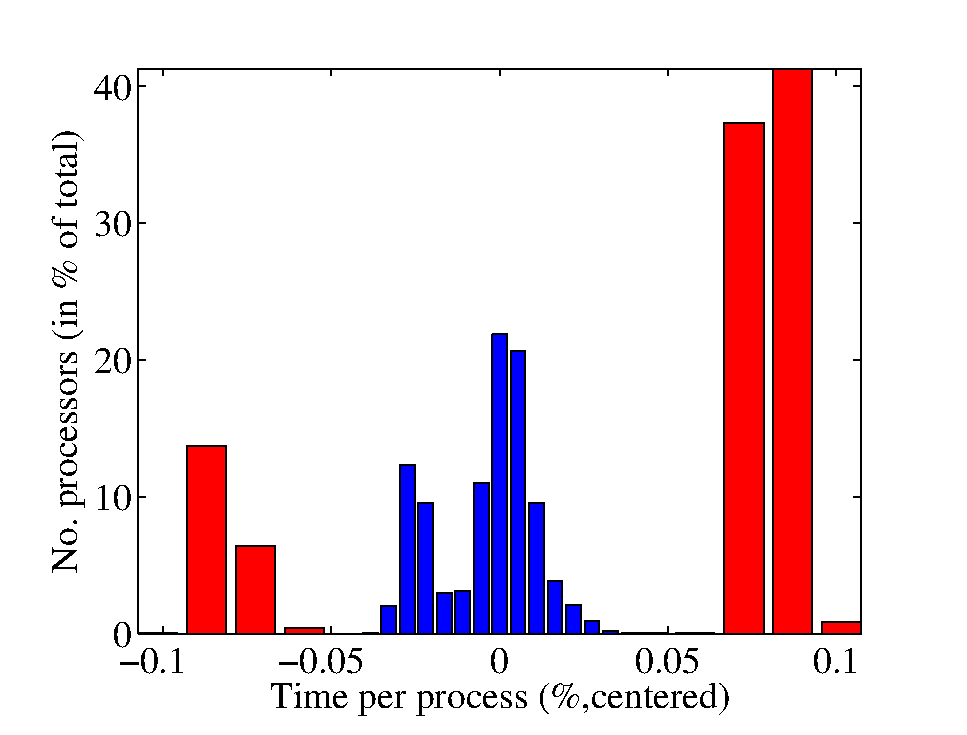
\includegraphics[width=\linewidth]{./figures/loadbalance.eps}
  \caption{Histogram of the load imbalance at $2.184\times10^9$ degrees of freedom: number of processes per time spent in communication. Red bins:\% of processes at the lowest per core load, blue bins:\% of processes at highest per core load}
  \label{fig:imbalancehist}
\end{figure}


On Mira the communication is mostly latency bound with a small influence of the
bandwidth. This holds true for peer to peer communication as well as for the
all-reduce (see \reffig{fig:pingpong}).

Across the four test cases we can observe a weak scaling in
\reffig{fig:weakscaling}. It proves that the scaling on Mira is only dependent
on the ratio $\frac{n}{P}$. 
\begin{figure}
  \centering
  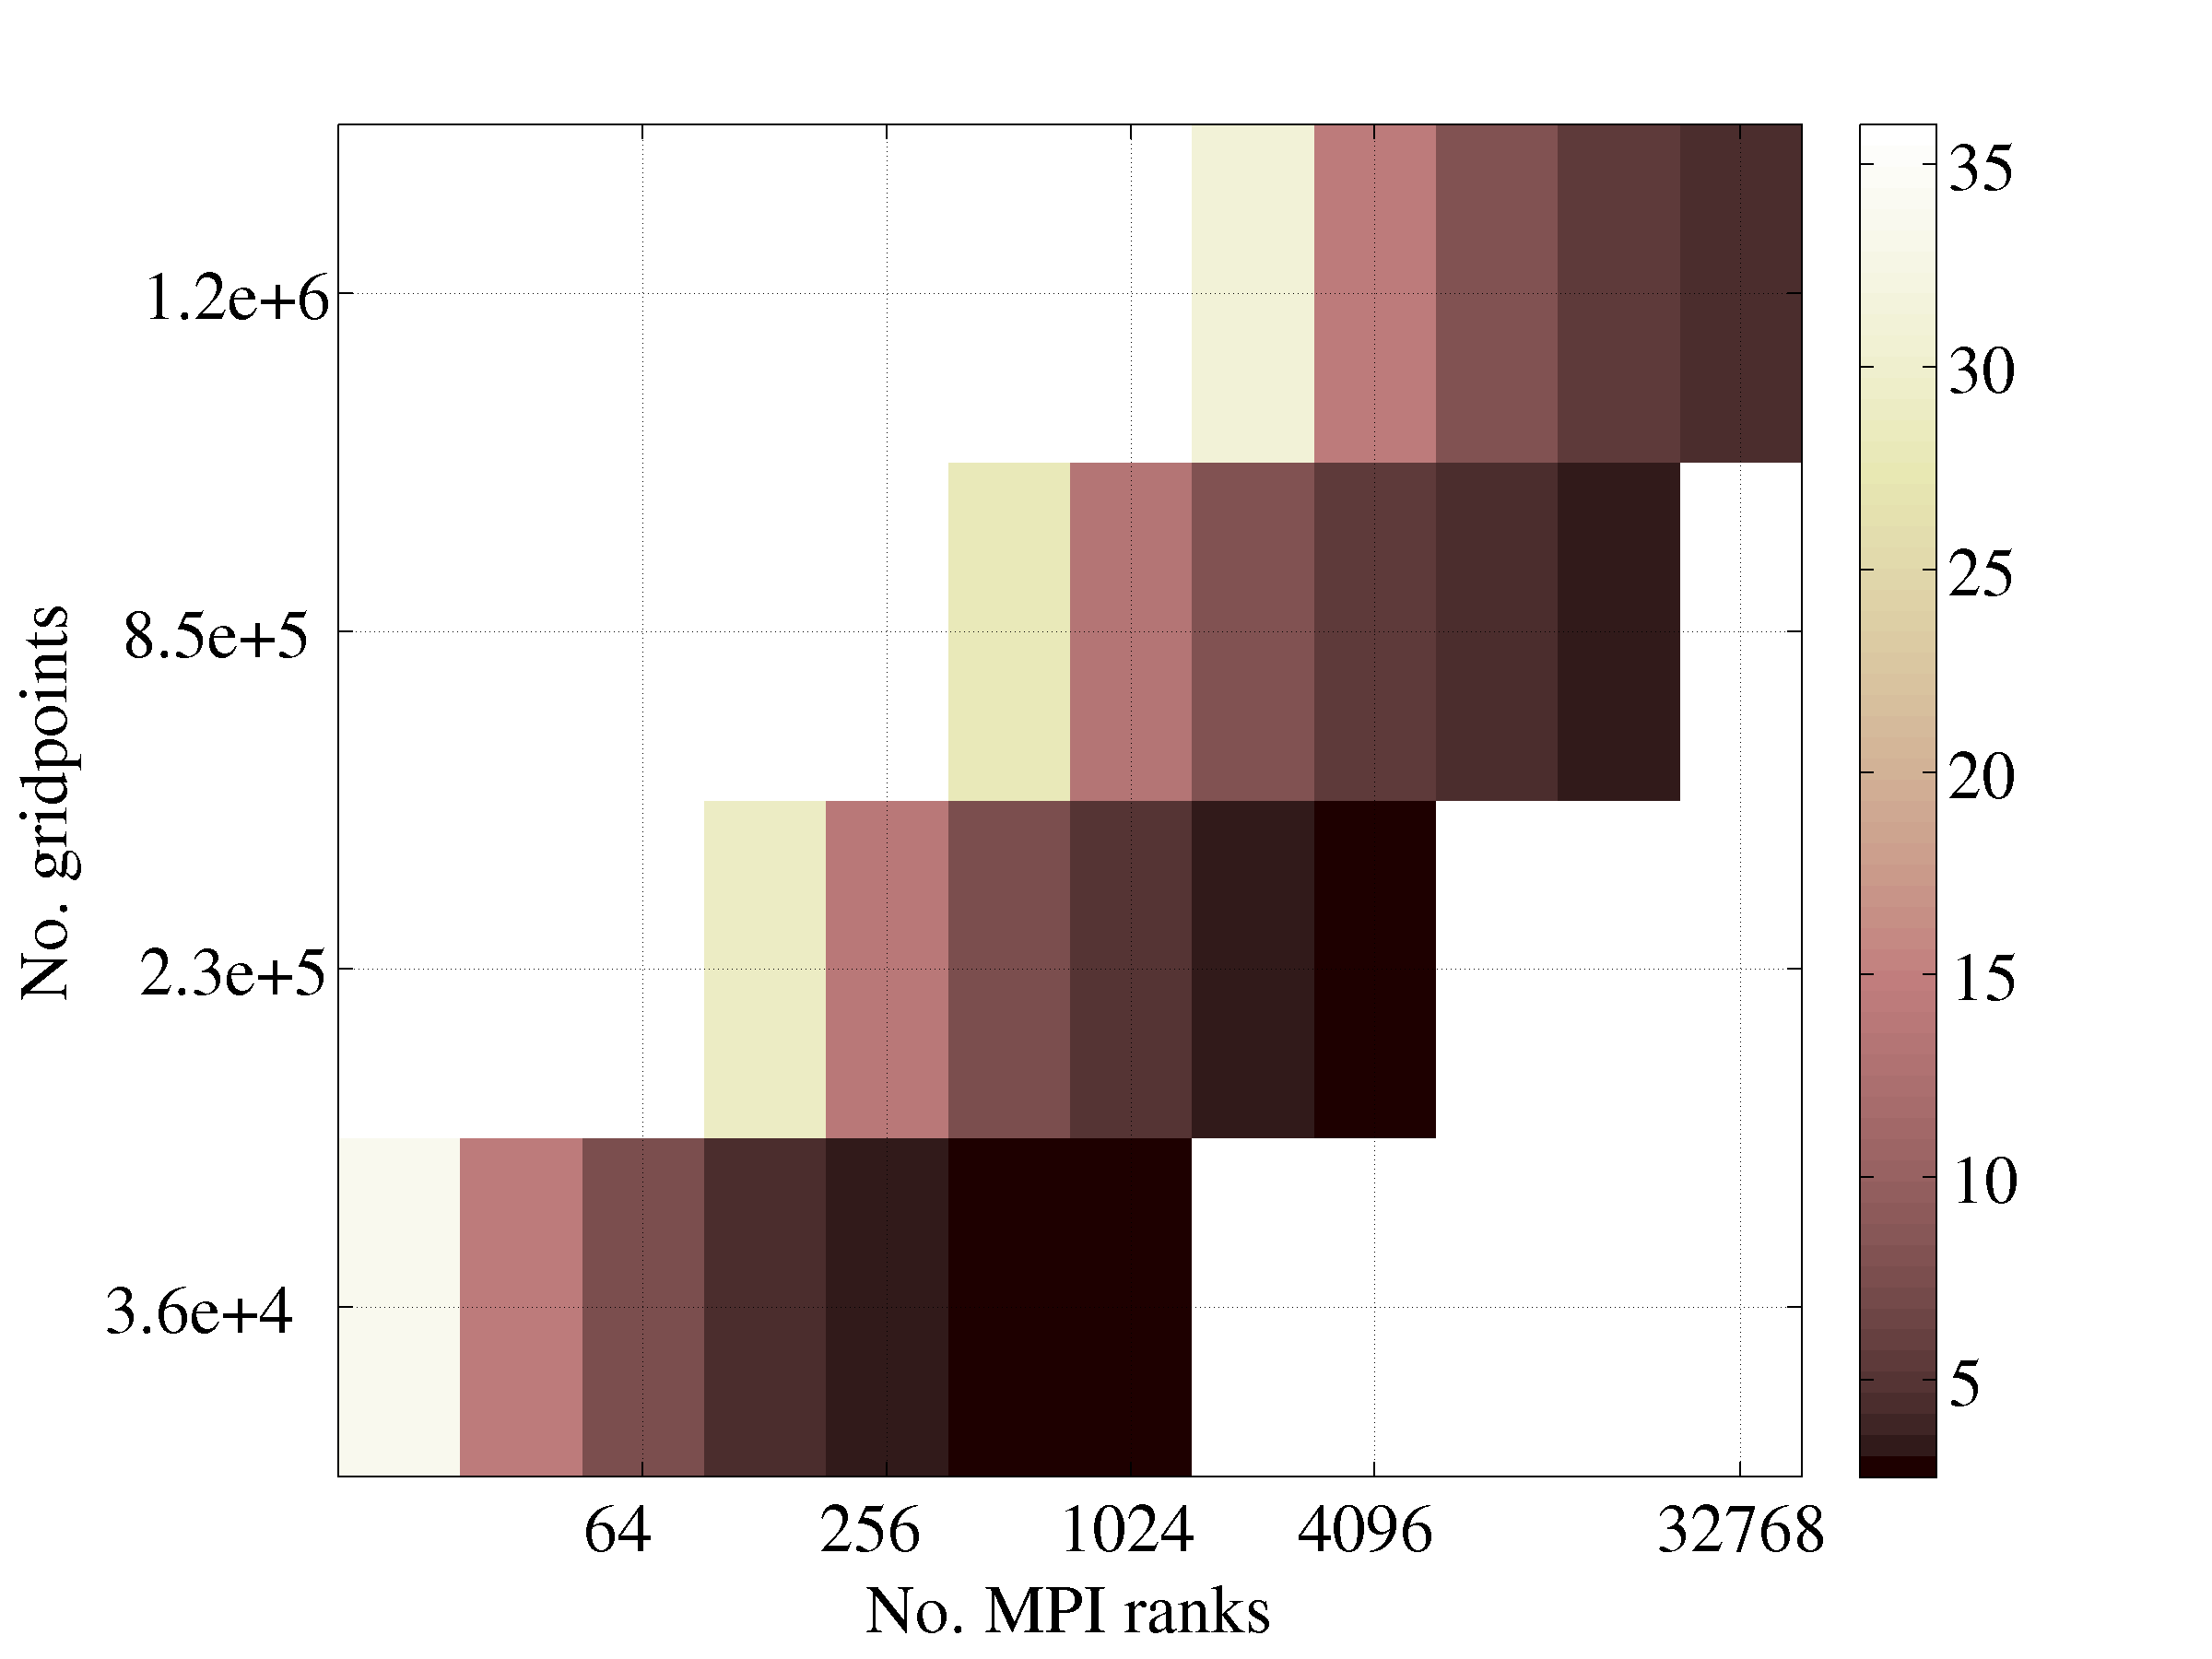
\includegraphics[width=\linewidth]{./figures/weak.png}
  \caption{Weak Scaling}
  \label{fig:weakscaling}
\end{figure}

\begin{figure}
  \centering
  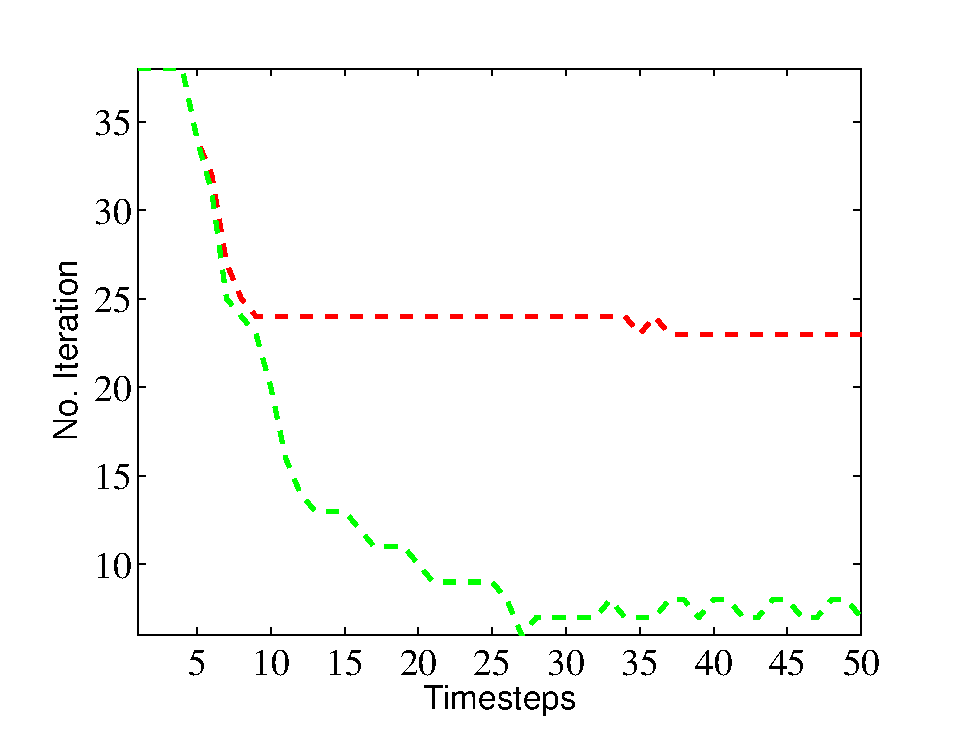
\includegraphics[width=\linewidth]{./figures/projections.eps}
  \caption{Convergence of solution with increase of projections space $L$. (green: $L=20$, red $L=0$) }
  \label{fig:projections}
\end{figure}
% Beskow

On Beskow, superlinear scaling is also visible over a large range of cores in \reffig{fig:scaling_beskow}. This shows once again the good strong scaling of Nek5000. We do not possess profiling results for Beskow and cannot study the cache misses but we assume that the reason for superlinearity is similar as for Mira. The scalability limit $r=1$ is more delicate to locate accurately because of the high variance in communication times (see \reffig{fig:pingpong_beskow}). We nevertheless present the scalability limit for the particular results from \reffig{fig:scaling_beskow} while keeping in mind that the intersection point would probably move significantly if the test had to be run again, depending on the nodes allocation, network traffic on the computer... However, we note that the scalability limit on Beskow is roughly one order of magnitude higher as on Mira in terms of degrees of freedom per core and $r=1$ is obtained at about $\frac{n}{P} \sim 20000 - 50000$. This is consistent with the values for the non-dimensional latency and inverse bandwidth from Table \reffig{tab:computer_charac} and the fact that Beskow has faster CPUs.
NOTE: Finish results analysis and comment on weak scaling when data for 16k and 32k available.

% Titan

Superlinear scaling occurs on Titan as well as we see in \reffig{fig:scaling_titan} and cache misses is once more assumed to be the reason. On the other hand, the scalability limit for this computer exhibits a different behaviour and the the number of degrees of freedom per core where $r=1$ increases significantly with bigger cases as we see from Table \reffig{tab:stronglimit}. The limit goes from $\frac{n}{P} \sim 9000$ to $\frac{n}{P} \sim 228000$ between the cases $Re_{\tau}=180$ and $Re_{\tau}=1000$ for XXT. It goes from $\frac{n}{P} \sim 11000$ to $\frac{n}{P} \sim 132000$ between the cases $Re_{\tau}=180$ and $Re_{\tau}=1000$ for AMG. This result means that despite good strong scaling, weak scaling is not obtained on Titan.


\section{Conclusion}
%\end{document}  % This is where a 'short' article might terminate
Our four test cases from 18 million to 2 billion degrees of freedom were
successfully run on three different petscale system architectures from the
lowest, memory bound, processor count to the granularity limit in order to
assess the strong scaling of Nek5000. On Mira we can confirm the theoratical
limits established in \cite{fischer:scaling} to match our results in the order
of magnitude. On the Cray systems we observed one to two orders of magnitude
lower strong scaling limits due to by an equally order of magnitude higher
latency and high noise in the network communication. We investigated the new
and updated projections and observed a much better behavior compared to past
implementations. Our results point at the regimes under which to chose AMG or
XXT; AMG for low latency and high element count, XXT for high latency, high
bandwidth and low element count. 

%ACKNOWLEDGMENTS are optional
\section{Acknowledgments}

%
% The following two commands are all you need in the
% initial runs of your .tex file to
% produce the bibliography for the citations in your paper.
\bibliographystyle{abbrv}
\bibliography{easc2016}  % template.bib is the name of the Bibliography in this case
% You must have a proper ".bib" file
%  and remember to run:
% latex bibtex latex latex
% to resolve all references
%
% ACM needs 'a single self-contained file'!
%
%APPENDICES are optional
%\balancecolumns
%\appendix
%Appendix A
%\section{Appendix A}
%\label{sec:plots}
% This next section command marks the start of
% Appendix B, and does not continue the present hierarchy

%\balancecolumns % GM June 2007
% That's all folks!
\end{document}

